\documentclass[a4paper,11pt]{article}%

\usepackage{fullpage}%
\usepackage[T1]{fontenc}%
\usepackage[utf8]{inputenc}%
\usepackage[main=english,francais]{babel}% % Adjust the main language

\usepackage{authblk}

\usepackage{amsfonts,amsmath,amssymb}%
\usepackage{amsthm}%

\usepackage{graphicx}%
\usepackage{subcaption}%
\usepackage{url}%
\usepackage{abstract}%

\usepackage{amsmath}%
\usepackage{subfig}%
\usepackage{color}

\usepackage{newpxtext, newpxmath}

\usepackage{mathpazo}%

\usepackage{array}

\usepackage{algorithm}
\usepackage{algorithmic}

\usepackage{tikz}
\usepackage{tikz-qtree}
\usepackage{forest}

\usepackage{xspace}

\usetikzlibrary{shapes}
\usetikzlibrary{calc}

% Configuration of the theorem style %

\newtheorem{thm}{Theorem}[section]%
\newtheorem{cor}[thm]{Corollary}%
\newtheorem{lem}[thm]{Lemma}%

\theoremstyle{proposition}%
\newtheorem{proposition}[thm]{Proposition}%

\theoremstyle{definition}%
\newtheorem{definition}[thm]{Definition}%

\theoremstyle{remark}%
\newtheorem*{remark}{Remark}%

\theoremstyle{example}%
\newtheorem*{example}{Example}%

\renewcommand\qedsymbol{$\blacksquare$}%

\newsubfloat{figure} % Subfigures


% \usepackage{listings}%

% \lstset{%
%   basicstyle=\sffamily,%
%   columns=fullflexible,%
%   language=C++,%       % Adjust according to your current language
%   frame=lb,%
%   frameround=fftf,%
% }%

\parskip=0.5\baselineskip

\sloppy

\begin{document}

\title{Potential NP-completeness of an approximate tree compression problem}

\author{Clément Legrand-Duchesne}

\affil{Univ Rennes, F-35000 Rennes, France}

\maketitle

\begin{abstract}
  A tree is said to be self-nested if all his subtrees of equal height
  are isomorphic. It has been shown that self-nested trees are a
  natural and relevant model for the structure of a plant. We are
  interested in approximating trees by self-nested trees. More
  precisely, given a tree $T$, we try to find the self-nested tree $S$
  that minimizes the edit distance between $S$ and $T$. In this paper,
  we present our attempts to prove that this problem is NP-complete,
  as well as polynomial algorithms when $T$ is of height 2.

  
  This internship has been carried out from May 28, 2018 to July 27,
  2018, in the MOSAIC team (MOrphogenesis Simulation and Analysis In
  siliCo) of the RDP laboratory (\emph{Reproduction et
    Développement des Plantes}) of the ENS de Lyon, under the
  supervision of Christophe Godin.

  \begin{description}
  \item[Keywords:] Graph Theory, NP-completeness, self-nested trees,
    edit distance, tree compression.
  \end{description}
\end{abstract}

\pagenumbering{gobble}

\tableofcontents 
\clearpage

\pagenumbering{arabic} % Start arabic numbering

\section*{Introduction}
\addcontentsline{toc}{section}{\protect\numberline{}Introduction}%

The MOSAIC team develops mathematical models and tools to study the
morphogenesis and growth of animals and plants. In order to do that,
they design mathematical models and data structures able to describe
efficiently and accurately the shapes and properties of the plants or
animals.

For example, it is natural to represent the branching structure of a
plant by a tree. In those trees representing plants, we can observe
that some ramifications patterns tend to repeat themselves in many
places. The MOSAIC team has thus designed a theoretical model of the
structure of a plant based on this idea of repeated patterns:
self-nested trees, trees in which all the subtrees of equal height are
isomorphic.

Some biological or physical quantities (such as the flow of sap in the
plant for example) can be computed on these trees. Depending on the
species, the size of the trees representing the plants can be
tremendous and lead to unreasonable computing time. They also
developed a compression algorithm for trees, based on the same idea of
patterns within the tree, by eliminating this redundancy. Moreover, by
eliminating this redundancy, the different patterns in the tree and
their organization are highlighted. For this reason, this compression
helps to understand the structure of the plant and its developement.

Those compression algorithms return DAGs (Directed Acyclic Graph) and
it is possible to show that the tree having the best compression
factor are the self-nested ones. Therefore, it is beneficial to
approximate trees by self-nested ones, in order to have an approximate
yet compact representation of them. There are several ways to do this
and the MOSAIC team has developed different algorithms doing
this. However, the approximation given by those algorithms are not the
best (either because these algorithms are heuristics or because some
additional conditions are imposed on the self nested trees returned by
the algorithm). In fact no efficient algorithm has been found to
compute the nearest self-nested tree to a tree.

Therefore, proving that there exists no polynomial algorithm solving
this problem would justify the use of the non optimal algorithms
previously developed by the team. More precisely, the goal of this
internship is to prove that this problem is NP-complete. NP-complete
problems are the hardest problems of the NP class and under the
assumption that the P and NP complexity classes are different, this
would prove there exists no polynomial algorithm able to find the
nearest self-nested tree to a tree in general.

The state of the art, along with definitions and notations will be
presented and introduced in a first section. We will then give further
details on the NP-complete theory and present the results found during
the intership. Finally, we will explain how this results consist in an
improvement of the state of the art and the consequences and
applications.

\section{Context}
\label{sec:context}
\subsection{Self-nested trees and definitions}

In this report, we will only consider rooted unordered trees, % which
% set will be 
denoted by $\mathcal{T}$. Unordered trees are trees for
which the order among the children of a same node is not significant.
Let $v$ be a node of $T$, the complete subtree of $T$ rooted in $v$ will be
denoted by $T[v]$.

Two trees $T_{1} = (V_{1},E_{1})$ and  $T_{2} = (V_{2},E_{2})$ are
said to be isomorphic if there exists a bijection $f$ from  
$V_{1}$ to  $V_{2}$ such that for each pair of nodes $(u,v)$ in  $V_{1}$,
$(u,v) \in E_{1}$ if and only if $(f(u),f(v)) \in E_{2}$.

Let us consider the equivalence relation $\equiv$ on $\mathcal{T}$
defined by $T_1 \equiv T_2$ if and only if $T_1$ and $T_2$ are
isomorphic. More generally, we will say that two nodes $v_1$ and 
$v_2$ of $T$ , are equivalent if the subtrees
$T[v_1]$ and $T[v_2]$ are isomorphic. We will denote the
equivalence class of $v$ by $C(v)$.

A self-nested tree is a tree whose subtrees of identical height are
isomorphic to one another. An exemple of tree that is not self-nested
is given Figure \ref{fig:treeexample}, an example of self-nested tree is given
Figure \ref{fig:SNtree}.  We will denote $\mathcal{S}$
the set of the self-nested trees.

\begin{figure}[h]
 \begin{subfigure}[b]{0.45\textwidth}
    \centering  
    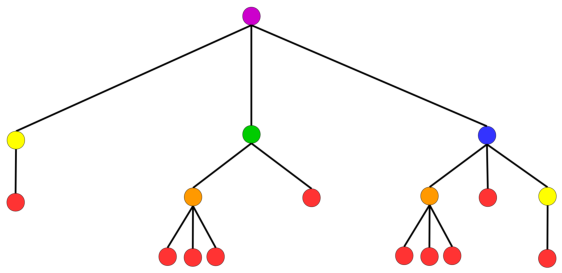
\includegraphics[width=\textwidth]{figures/tree2.pdf}
    \caption{Example of regular tree}
    \label{fig:treeexample}
  \end{subfigure}
  \quad
  \begin{subfigure}[b]{0.45\textwidth}
    \centering  
    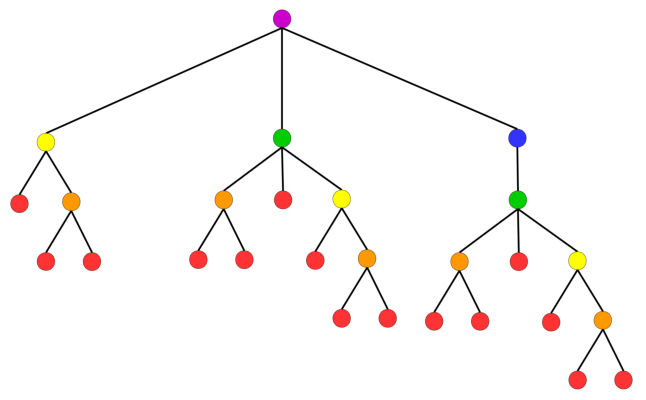
\includegraphics[width=\textwidth]{figures/tree.pdf}
    \caption{Example of self-nested tree}
    \label{fig:SNtree}
  \end{subfigure}
 
  \caption{Difference between regular trees and self nested trees}
\end{figure}

\subsection{DAG compression}

For $T = (V,E) \in \mathcal{T}$, let 
$\mathcal{Q}(T) = (V_{\mathcal{Q}}, T_{\mathcal{Q}})$ be the quotient
graph of $T$
by the equivalence relation $\equiv$. In concrete terms,
$V_{\mathcal{Q}} = \{ C(v) | v \in V \}$ is the quotient set of $V$ by
$\equiv$ and 
${E_{\mathcal{Q}} = \{ (C(u), C(v)) | (u,v) \in T \}}$.
Let $\delta$ be the weighting function on $\mathcal{Q}(T)$
defined by $$\delta(C(u), C(v)) = \#\{ v' \in Child(u) | C(v) = C(v')\}$$

The subfigure \ref{fig:dagexample} the quotient graph
corresponding to the tree represented Subfigure \ref{fig:treeexample}. The
equivalent nodes are represented in the same color.

\begin{figure}[h]
  \begin{subfigure}[b]{0.45\textwidth}
    \centering
    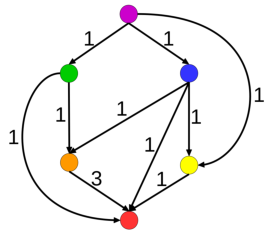
\includegraphics[width=.5\textwidth]{figures/dag2.pdf}
    \caption{DAG compression of the tree Subfigure \ref{fig:treeexample}}
    \label{fig:dagexample}
  \end{subfigure}
  \quad
  \begin{subfigure}[b]{0.45\textwidth}
    \centering
    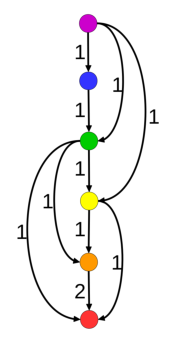
\includegraphics[width=.3\textwidth]{figures/dag.pdf}
    \caption{DAG compression of the tree Subfigure \ref{fig:SNtree}}
    \label{fig:SNdag}
  \end{subfigure} 
  \caption{Example of DAG compression}\label{fig:example}
\end{figure}

Let $T \in \mathcal{T}$, C. Godin and P. Ferraro showed in
\cite{godin} that $\mathcal{Q}(T)$ is a weighted directed acyclic
graph (\emph{DAG}) and that for each \emph{DAG} $Q$ with a weighting
function $\delta$, there exists a single tree $T \in \mathcal{T}$ such
as $\mathcal{Q}(T) = Q$.

The trees whose quotient graph is a linear \emph{DAG} (\emph{DAG} for
which there exists a hamiltonian path) are exactly the self-nested
trees. Since the nodes of equal height in a self-nested tree are
isomorphic to one anoter, there is a single vertex in the \emph{DAG}
for each height: the tree Subfigure \ref{fig:SNdag} is the quotient
graph of the self-nested tree represented Subfigure
\ref{fig:SNtree}. As a result, the number of vertices in the
\emph{DAG} is equal to the height of the initial tree.

\subsection{Avantages of self-nested trees}

Self-nested trees have a linear quotient graph, as a result they are
cheaper to store, but there are other advantages...

Let $T \in \mathcal{T}$ and $f$ be a recursive function ($f(u)$ depends
only on the values $(f(u_{i}))_{i \in I}$ where $(u_{i})_{i \in I}$
are the children of $u$). For example, $f$ can be the height or the
number of vertices of the subtree rooted in $u$. Since $f$ is
recursive, $f$ takes the same value on all the subtrees of $T$
isomorphic to one another, and computing $f$ on $T$ leads to make the
same computation several times. Thus, computing $f(T)$ directly on the DAG
corresponding to $T$ is more efficient than computing it on $T$ itself.

For example on Figure \ref{fig:compute} we can compute the number of
nodes directly on the DAG: the number of nodes under a leaf (red node)
is equal to one, the number of nodes under the orange nodes in $T$ is
equal to three times the number of nodes under a leaf plus one, that
is four. We can carry one the computation, at the end the number of
recursive calls will be equal to the number of nodes in the DAG
instead of the number of nodes in the tree (as it would have been if
we had computed $f$ on the tree).  Thus, the computation of recursive
functions is particularly efficient on self-nested trees because of the
small size of their DAG.

\begin{figure}[h]
  \centering
  \begin{subfigure}[b]{0.5\textwidth}
    \centering  
    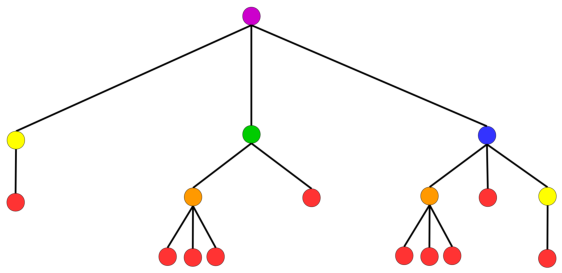
\includegraphics[width=\textwidth]{figures/tree2.pdf}
    \caption{Example of tree}
  \end{subfigure}
  \quad 
  \begin{subfigure}[b]{0.4\textwidth}
    \centering
    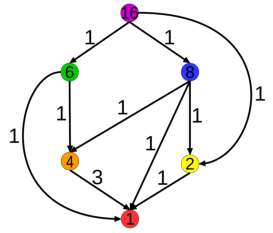
\includegraphics[width=.7\textwidth]{figures/dag2_nb_node.pdf}
    \caption{Computation of the number of nodes directly on its DAG}
    \label{fig:computeondag}
  \end{subfigure}
  \caption{Example of computation on the DAG}\label{fig:compute}
\end{figure}

Self-nested trees are a particularly relevant model of the structure
of a plant and are therefore usefull for the study of their
growth. Indeed, meristems are the tissues responsible for the growth
and some studies support the idea that the meristems of a plant go
through successive developement stages during their lives
\cite{meristems}. Furthermore, the transitions from one stage to
another occur in the same way for all the meristems of a same plant
and are specific to the species. We can indeed observe that the way
plants grow, the branching structure of their stems and branches seem
to follow some regular pattern repeated in several places in the
plant. Thus, representing the structure of the plant by a self-nested
tree whose nodes are the meristems and edges are the stems or branches
of the plant is natural and appropriate.

Unfortunately, a real plant has few chances to have exactly the
structure of a self-nested tree. Indeed, environmental conditions
(such as light and nutrition for example) also impact the growth of
the plant. This is one of the reasons why we are interested in
approximating trees by self-nested ones.

\subsection{Edit distance}
Let us consider the two following edit operations: the deletion and
addition of a node. Deleting a node $u$ in a tree means making the
children of $u$ children of the father of $u$ before removing $u$ from
the tree (Figure \ref{fig:deletion}). Adding a node is the
complementary operation, thus adding a node $u$ under $v$ means making
a subset of the children of $v$ become children of $u$ before placing
$u$ under $v$ (Figure \ref{fig:addition}).

\begin{figure}[h]
  \centering
  \begin{subfigure}[b]{0.3\textwidth}
    \centering  
    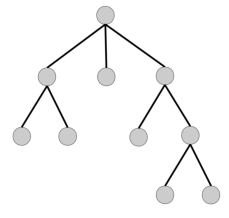
\includegraphics[width=.8\textwidth]{figures/edit.pdf}
    \caption{Initial tree}
  \end{subfigure}
  \begin{subfigure}[b]{0.3\textwidth}
    \centering
    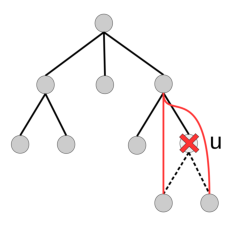
\includegraphics[width=.8\textwidth]{figures/edit_deletion.pdf}
    \caption{Deleting a node}
    \label{fig:deletion}
  \end{subfigure}
  \begin{subfigure}[b]{0.3\textwidth}
    \centering
    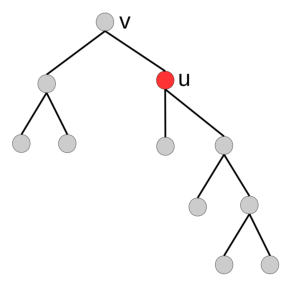
\includegraphics[width=\textwidth]{figures/edit_addition.pdf}
    \caption{Adding a node}
    \label{fig:addition}
  \end{subfigure}
  \caption{Example of edit operations}\label{fig:edit}
\end{figure}

Let $T_{1} = (V_{1},E_{1})$ and $T_{2} = (V_{2},E_{2})$ be two
trees. 

An edit sequence is a succession of edit operations. We can define the
cost of an edit sequence by the number of edit operations that were done.

An edit mapping between $T_{1}$ and $T_{2}$ is
a function $\Phi : V'_{1} \rightarrow V'_{2}$ where
$V'_{1} \subseteq V_{1}$ and $V'_{2} \subseteq V_{2}$, such as $\Phi$
is a bijection and preserves ancestrality among the nodes (in other
words, $u \in V'_{1}$ is an ancestor of  $v \in V'_{1}$ if and only if
$\Phi(u)$ is an ancestor of $\Phi(v)$). 

Given an edit mapping $\Phi$ between $T_{1}$ and $T_{2}$, there exists
a natural edit sequence leading from $T_{1}$ to $T_{2}$: every node
belonging to $V_{1} \setminus V'_{1}$ is deleted and every node in
$V_{2} \setminus V'{2}$ is added. Thus, we can define the cost of an
edit mapping $\Phi$ as the number of nodes that were added or deleted:
${\#(V_{1} \setminus V'_{1}) + \#(V_{2} \setminus V'_{2})}$.

More precisely, K.Zhang showed in \cite{zhang} that for every edit
mapping between $T_{1}$ and $T_{2}$ there exists a edit sequence of
equal cost. He also showed that for every edit sequence of $k$
operations leading from $T_{1}$ to $T_{2}$, there exists an edit
mapping of cost less than $k$.

It is also possible to define the edit distance between the trees
$T_{1}$ and $T_{2}$ as the minimal cost of an edit mapping between the
two trees (the properties of symmetry, identity of indescernibles and
triangle inequality are satisfied). We will notice that the minimal
cost of an edit mapping between $T_{1}$ and $T_{2}$ is also the
minimal cost of an edit sequence leading from $T_{1}$ to $T_{2}$
(result from the preceding properties shown in \cite{zhang}). 

In \cite{NPCzhang} K. Zhang, R. Statman and D. Shahsha show that the
problem of computing the edit distance between two trees is
NP-complete. There are several ways to overcome this difficulty: one
of them consists in restricting the set of instances to consider a set
of trees in which the distance is easier to compute. Another one consists
in modifying slightly the distance, for example by adding other
constraints, in order to build a new edit distance easier to compute.

The article \cite{zhang} presents an additional, sufficient and not
very constraining condition on the edit mapping along with a
polynomial algorithm to compute the new distance. The condition on the
edit mapping is the following: for all $u,v,w \in V'_{1}$, the least
common ancester of $u$ and $v$ is a proper ancester of $w$ if and only
if the least common ancestor of $\Phi(u)$ and $\Phi(v)$ is a proper
ancestor of $\Phi(w)$. In other words, $\Phi$ preserves the sibling
relation among the nodes: a node can be deleted only if all his
descendant are deleted as well or if all his siblings have been
deleted; during the addition of a new node $u$ under $v$, all the
children of $v$ have to become children of $v$ or none of them.

In this article, we will use this edit distance with its new
constraint.

\subsection{Approximation by self-nested trees}

As we explained before, a real plant has few chances to have an exact
self-nested structure. Therefore, approximating the trees of the
structure of different plants by self-nested trees could allow us to
find the theorical growth model of each species and thereby lead to a
better understanding of the evolution of the meristems.

If the goal is to compute the value taken by a recursive function $f$
on a tree $T$, approximating $T$ by a self-nested tree $S$ allows us to
compute very effectively $f(S)$, which can, under certain conditions,
be an approximative value of $f(T)$. 

\begin{figure*}
  \centering
  \begin{subfigure}[b]{0.475\textwidth}
    \centering
    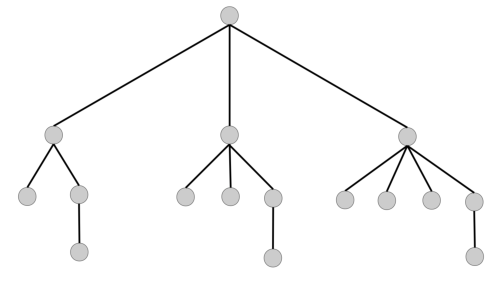
\includegraphics[width=\textwidth]{figures/T.pdf}
    \caption{$T$}    
    \label{fig:T}
  \end{subfigure}
  \hfill
  \begin{subfigure}[b]{0.475\textwidth}  
    \centering 
    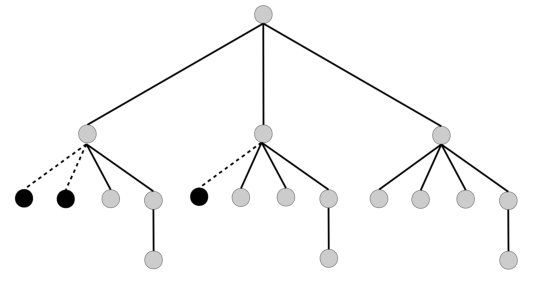
\includegraphics[width=\textwidth]{figures/NEST(T).pdf}
    \caption{$NEST(T)$}    
    \label{fig:NEST(T)}
  \end{subfigure}
  \vskip\baselineskip
  \begin{subfigure}[b]{0.475\textwidth}   
    \centering 
    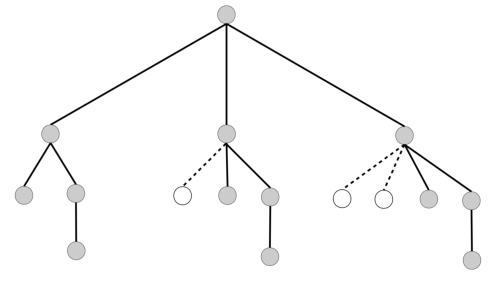
\includegraphics[width=\textwidth]{figures/NeST(T).pdf}
    \caption{$NeST(T)$}    
    \label{fig:NeST(T)}
  \end{subfigure}
  \quad
  \begin{subfigure}[b]{0.475\textwidth}   
    \centering 
    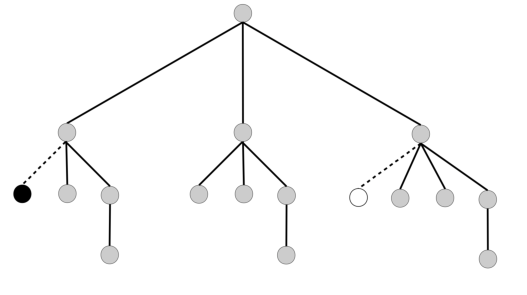
\includegraphics[width=\textwidth]{figures/NST(T).pdf}
    \caption{$NST(T)$}    
    \label{fig:NST(T)}
  \end{subfigure}
  \caption{Different approximations of $T$ by self-nested trees} 
  \label{fig:approx}
\end{figure*}
    
Several meanings can be given to the term ``approximating a tree by a
self-nested one''. For example, C. Godin and P. Ferraro have proposed a
polynomial algorithm \cite{godin} to compute the NEST (Nearest
Embedding Self-nested Tree) of a tree $T$. The NEST of $T$ is the
self-nested tree $S$ that minimize the edit distance between $S$ and
$T$ and that embeds $T$. It can also be described as the minimal
self-nested tree embedding $T$ and it can be obtained only by doing
adding operations on $T$.
For example, the NEST of $T$ (Figure \ref{fig:T}) is given in Figure
\ref{fig:NEST(T)}. The black nodes are the added ones. $T$ is at
distance 3 from its NEST. 

R. Azais then presented an algorithm \cite{romain} computing in
polynomial time the NeST (Nearest embedded
Self-nested Tree) of a tree $T$. The NeST of $T$ is the self-nested tree $S$ that
minimize the edit distance between $T$ and $S$ and is embedded in
$T$. It is the maximal self-nested tree embedded in $T$ and it can be
obtained only by deleting nodes from $T$. %insérer image 
For example, the NeST of $T$ (Figure \ref{fig:T}) is given in Figure
\ref{fig:NeST(T)}. The white nodes are the ones that are deleted. $T$
is at distance 3 from its NeST. 

The NST (Nearest Self-nested Tree) of a tree $T$ is the self-nested
tree $S$ that minimize the edit distance between $T$ and $S$
(authorizing this time both adding and deleting operations)
\cite{godin}.  For example, the NST of $T$ (Figure \ref{fig:T}) is
given in Figure \ref{fig:NST(T)}. The white node is the one that is
deleted and the black node is the one that is added. $T$ is at
distance 2 from its NST.

No polynomial algorithm able to compute the NST of a tree has been
found yet. Thus, the goal of the internship is to prove that there
exists no such algorithm (more precisely that the NST problem is
NP-complete). This result would justify the use of approximation
algorithms such as the heuristic and the algorithm computing the NeST
and the NEST.

\newcommand\variable{\emph{variable}\xspace}
\newcommand\variables{\emph{variables}\xspace}
\newcommand\widget{\emph{widget}\xspace}
\newcommand\widgets{\emph{widgets}\xspace}
\newcommand\constraint{\emph{constraint}\xspace}
\newcommand\constraints{\emph{constraints}\xspace}
\newcommand\Variable{\emph{Variable}\xspace}
\newcommand\Variables{\emph{Variables}\xspace}
\newcommand\Widget{\emph{Widget}\xspace}
\newcommand\Widgets{\emph{Widgets}\xspace}
\newcommand\Constraint{\emph{Constraint}\xspace}
\newcommand\Constraints{\emph{Constraints}\xspace}

\section{Contribution}

We assume that the reader is familiar with the complexity theory. In
this article, we will denote the set of instances by $\Omega$ and the
set of positive instances by $Y$. See the appendix for further
reminder on the complexity theory.

I did not manage to prove that the NST problem is NP complete. We will
also present in this section the different attempts we made and the
reasons why they were relevant but not conclusive. 

\subsection{Belonging to the NP class}

We aim to prove that the NST decision problem is NP-complete, this
means it would belong to the NP class and be NP-hard. It
clearly belongs to the NP class. Indeed, for all tree $T = (V,E)$, for
all integer $k$, given a potential solution $S$, it is possible to
ascertain whether or not $S$ is self-nested, and to compute the
distance between $S$ and $T$, both in polynomial time.

%%%%%%%%%%%%%%%%%%%%%%%%%%%%%%%%%%%%%%%%%%%%%%%%%%%%%%%%%%%%%%%%%%%%%%%%%%%%
\noindent\hrulefill

\subsection{First approach}
To help us build the reduction, a few conceptual remarks can be made,
in order to guide the research. First of all, the reduction has no
obligation to be surjective; as a matter of fact, it is quite often
not surjective. Indeed, in order to be able to prove the equivalence
$\omega_{A} \in Y_{A} \Leftrightarrow \omega_{B} = f(\omega_{A}) \in
Y_{B}$
(where $A$ is the initial NP-complete problem and $B$ is the problem
we consider), the images of the reduction have often a very
particular shape. Yet, the image of $\Omega_{A}$ by the reduction has
to be big enough so that we are unable to find a polynomial algorithm
solving the problem on the set of images of the reduction. Indeed,
finding such an algorithm and a reduction would mean we would have
solved the open question of the equality of the P and NP classes,
which is unreasonable.

In order to understand better the difficulty of the problem, I tried
to find a way to compute efficiently the NST in special cases. Indeed,
as long as we find a polynomial algorithm solving the NST problem on
the set of trees considered, we are ensured that the difficulty
leading to the NP-hardness lies somewhere else. I also decided to
start with very special cases where polynomial algorithms could be found
and to add progressively some generality to identify the trees and
conditions that make the problem difficult. 

I first considered the trees of height 2. In the NEST and NeST
algorithms, C. Godin, P. Ferraro and R. Azais consider only edit
operations such that the height of any pre-existing node is unchanged
(see Figure \ref{fig:edit_height}). For the sake of simplicity, I
decided to first use these edit operations.

\begin{figure}
  \centering
  \caption{edit operation height conservation}
  \label{fig:edit_height}
\end{figure}

\subsubsection{Trees of height 2 with height conservation} 
Let $T$ be a tree of height 2 (see Figure \ref{fig:height2}). Let us
denote $NST(T)$ by $S$ and an optimal edit mapping between $T$ and $S$
by $\Phi$. We will show in this section that it is possible to find
$\Phi$ and $S$ in polynomial time.  

We can first notice that if there are any leaves of depth 1, they do
not require any edit operations to obtain $NST(T)$. We can for this
reason assume that every node of depth 1 is of height 1 (see Figure
\ref{fig:height2}).

\begin{figure}
  \centering
  \includegraphics[width=.4\textwidth]{figures/tree_height2.pdf}

  \caption{example of tree of height 2}
  \label{fig:height2}
\end{figure}

Let us denote the nodes of height 1 of $T$ by
$(u_{i})_{1 \leqslant i \leqslant N}$ and
$(n_{i})_{1 \leqslant i \leqslant N}$ their respective number of
children. We will suppose that the sequence
$(n_{i})_{1 \leqslant i \leqslant N}$ is sorted by ascending
order. Each $u_{i}$ can be either deleted or mapped on a node of
height 1 in $S$, and since $S$ is self-nested, all the nodes of height
1 in $S$ are isomorphic to one another. The complete subtree under
each node of height 1 of $S$ is characterized by its number of
leaves. As a result, the edit mapping leading from $T$ to $S$ is
characterized by the $I_{0}$ the set of indices of the nodes deleted
and by $\tilde{n}$ the number of leaves under a node of height 1 in
$S$. Thus, we will try to find $I_{0}$ and $\tilde{n}$ such that the
corresponding self nested tree is a minimal distance from $T$.

Because of the constraint of Zhang, before deleting one of the nodes
$u_{i}$ of height 1 in $T$, it is necessary to delete all of his
children except one. Therefore, deleting $u_{i}$ costs $n_{i}$ where
$n_{i}$ is the number of children of $u_{i}$.

If $u_{i}$ is not deleted, than we have to adjust the number of
children it has to $\tilde{n}$, which costs
$\left|n_{i} - \tilde{n}\right|$. As a result, $u_{i}$ has to be
deleted if and only if $n_{i}$ is closer to 0 than to
$\tilde{n}$. Figure \ref{fig:optimalcost} shows $f_{i}$ the minimum
cost for each $u_{î}$ in function of $\tilde{n}$.

We will denote by $I_{1}$ the complement of $I_{0}$ in the set of
indices $\llbracket 1;N \rrbracket$. $I_{1}$ is composed of the
indices $i$ such that $\Phi(u_{i})$ is of height 1.
\begin{remark}
  The distance between $T$ and $S$ is equal to $\sum_{i \in I_{0}}
  n_{i} + \sum_{i \in I_{1}} \left| n_{i} - \tilde{n} \right|$
\end{remark}

\begin{figure}
  \centering
  \caption{optimal cost for $u_{i}$ in function of $\tilde{n}$}
  \label{fig:optimalcost}
\end{figure}

By summing the functions $f_{i}$ on every $u_{i}$, we obtain $f$ the
minimal cost of a mapping leading from $T$ to a self nested tree of
height 2, with $N$ nodes of depth 1, in function of $\tilde{n}$ the
number of children of the nodes of height 1. We can observe that the
resulting function is a piecewise linear function and that every break
in its differentiability has for abscissa one of the $n_{i}$ or
$2*n_{i}$. Therefore, the minimum of this function is reached in one
of those points. Since every $f_{i}$ is increasing just before
$2*n_{i}$ and constant after and that the derivative of the other
$f_{j}$ are equal before and after $2*n_{i}$, $2*n_{i}$ cannot be a
minimum of $f$.

Thus, by evaluating $f$ on every $n_{i}$, it is possible to find the
minimum of $f$ and thereby find the NST of $T$.

It is possible to show that every $f(n_{i})$ can be computed in
constant time by using the value of $f(n_{i-1})$. $f(n_{1})$ can be
computed in linear time. For this reason, $NST(T)$ can be computed in
$O(N*log(N))$ (it is necessary to order the
$(n_{i})_{1 \leqslant i \leqslant N}$ by ascending order) where $N$ is
the number of nodes of height 1 in $T$.

Since the NST (with only height preserving operations) can be computed
in polynomial time on the trees of height 2, this proves that if the
NST problem (with only height preserving operations) is NP-complete,
the set of images of the reduction cannot be the trees of height 2,
otherwise we would have found a way to solve any NP-complete problem
in polynomial time, which is unreasonnable.

We can make two more remarks that will help us later. 

\begin{remark} 
  For every $i \in I_{0}$, for
  every $j \in I_{1}$, $n_{i} < n_{j}$.\\
  Intuitively, if $n_{i} < n_{j}$ it costs less to delete all the
  children of $u_{i}$ than the one of $u_{j}$. See appendix for the proof.
\end{remark}

\begin{remark}
  Furthermore, $\tilde{n}$ is one of the medians of the
  $(n_{i})_{i \in I_{1}}$. \\
  Indeed, the median minimizes
  $\sum_{i \in I_{1}} \left| n_{i} - \tilde{n} \right|$. See proof in
  appendix for further details.
\end{remark}

We will keep in mind that the solution that we proposed here is a
brute-force search, we didn't manage to find any strategy that would
help us understand why computing the NST of a tree of height 2 seems
to be easier than in the general case. The main reason that explains
why this special case is easy to solve is that the trees of height 2
are simple enough to have a NST described by only 2 parameters.

\subsubsection{Trees of height 2 without preserving the height of the
  nodes}

The NST problem is solved easily on the trees of height 2 if we
authorize only the edit operations preserving the height. It can
either be due to the set of trees considered or to the restriction on
the edit operations. To gain in generality, I decided to look at the
problem without the restriction on the edit operations, in order to
use the work done in the previous section. Once again, I couldn't find
any global stategy that would give us a polynomial algorithm so I
tried to find as many properties on the NST of $T$ as I could, in
order to reduce the space of possibilities that we have to explore.

Since the poofs are quite fastidious we will only present the results
we found in this section, the poofs of the lemmas are in the appendix.

We will use the same notations as in the preceding paragraph. We will
denote by $I_{k}$ the set of indices $i$ of
$\llbracket 1;N \rrbracket$ such that $\Phi(u_{i})$ is of height
$k$. Let us denote by $\tilde{n}^{k}$ the number of children of the
nodes of height $k$ in $S$.

It is possible to show that $S$ has the shape depicted Figure
\ref{fig:shape_NST_2} %inserer figure
and that $S$ is characterized by
$(I_{k})_{0 \leqslant k \leqslant H-1}$ and
$(\tilde{n}^{k})_{1 \leqslant k \leqslant H-1}$ where $H$ is the
height of $S$. Therefore, the goal is to find the families
$(I_{k})_{0 \leqslant k \leqslant H-1}$ and
$(\tilde{n}^{k})_{1 \leqslant k \leqslant H-1}$ suh that the
corresponding self nested trees is at minimal distance from $T$.
\begin{figure}
  \centering
  
  \caption{Shape of $S$}
  \label{fig:shape_NST_2}
\end{figure}
The remarks of the previous section can be adapted.

\begin{lem}
  \label{lem:increasn}
  For every $k \geqslant 0$, for every $i \in I_{k}$ and $j \in
  I_{k+1}$, $n_{i} < n_{j}$.
\end{lem}

\begin{lem}
 The distance between $T$ and $S$ is equal to 
 $$ D(S,T) = \sum_{i \in I_{0}} n_{i} + \sum_{k = 1}^{H} \left(
   \sum_{i \in I_{k}} |n_{i} - \tilde{n}^{k}| + |I_{k}|\sum_{l =
     1}^{k-1}(\tilde{n}^{l}) \right)$$ 
 which is also equal to 
 $$ D(S,T) = \sum_{i \in I_{0}} n_{i} + \sum_{k = 1}^{H} \left(
   \sum_{i \in I_{k}} |n_{i} - \tilde{n}^{k}| + \tilde{n}^{k}\sum_{l =
     k+1}^{H}(|I_{l}|) \right)$$
 \begin{proof}
   Let $i \in I_{0}$. $u_{i}$ is deleted, which costs $n_{i}$ (as
   explained in the previous section).\\
   Let $i \in I_{k}$ with $k \geqslant 1$. $\Phi(u_{i})$ is of height
   $k$. To obtain the complete subtree under $\Phi(u_{i})$ in $S$ from
   the subtree under $u_{i}$ in $T$, it is necessary to adjust the
   number of children of $u_{i}$ to $\tilde{n}^{k}$ which costs
   $\left| n_{i} - \tilde{n}^{k} \right|$. It is also necessary to add
   $\sum_{l = 1}^{k-1}\tilde{n}^{l}$ nodes under one of the children
   of $u_{i}$, so that the height of $u_{i}$ increases to $k$.
   \end{proof}
\end{lem}

For every partition $(I_{k})_{0 \leqslant k \leqslant H-1}$ of
$\llbracket 1;N \rrbracket$, that verifies the lemma
\ref{lem:increasn}, it is possible to compute in $O(N)$ the family
$(\tilde{n}^{k})_{1 \leqslant k \leqslant H-1}$ such that the distance
between the corresponding self nested tree and $T$ is minimal. It is
also possible to show that

\begin{lem}
  \label{lem:ik}
  For every $k \geqslant 1$,
  $$|I_{k}| > \sum_{l = \ k+1}^{H-1} |I_{l}|$$
\end{lem}

\begin{lem}
  \label{lem:tilden}
  For every $k \geqslant 1$,
  $$\tilde{n}^{k} > \sum_{l = 1}^{k-1} \tilde{n}^{l}$$
\end{lem}
 
\begin{cor}
  The height $H$ of $S$ is bounded by $min(log_{2}(N+1),
  log_{2}(n_{N}+1))$.
  \begin{proof}
    The lemma \ref{lem:ik} leads to the following inequalities: 
    $$
    \begin{array}{rcl}
      |I_{k}| &\geqslant& \sum_{l=k+1}^{H} |I_{l}| + 1\\
              &\geqslant& |I_{k+1}| + \sum_{l=k+2}^{H} |I_{l}| + 1 \\
              &\geqslant& 2(\sum_{l=k+2}^{H} |I_{l}| + 1) \\
              &\geqslant& 2^{H-k-1}(I_{H} +1)\\
              &\geqslant& 2^{H-k}\\
    \end{array}
    $$
    As a consequence,
    $N \geqslant \sum_{k=1}^{H} |I_{k}| \geqslant \sum_{k=1}^{H}
    2^{H-k} \geqslant 2^{H} -1$,
    and $H \leqslant \left\lfloor \log_{2}(N+1) \right\rfloor$.\\
    The same reasonning can be applied to the lemma \ref{lem:tilden}
    to show that $H \leqslant \left\lfloor \log_{2}(\tilde{n}^{H}+1)
    \right\rfloor$, and we will notice that $\tilde{n}^{H} \leqslant
    n_{N}$, which leads to the result.
  \end{proof}
\end{cor}

By enumerating the partitions $(I_{k})_{0 \leqslant k \leqslant H-1}$
that verify the lemmas \ref{lem:increasn} and \ref{lem:ik} and
computing the optimal family
$(\tilde{n}^{k})_{1 \leqslant k \leqslant H-1}$ and the distance to
the corresponding self nested tree each time, we will find the NST of
$T$. The number of partitions $(I_{k})_{0 \leqslant k \leqslant H-1}$
of $\llbracket 1;N \rrbracket$ that verify the lemmas
\ref{lem:increasn} and \ref{lem:ik} is bounded by
$\frac{\binom{N+H}{H}}{2^H}$. 

Since $\frac{\binom{N+H}{H}}{2^H}$ is a $O(N^H)$ and that $H \leqslant
log_{2}(N)+1$, the number of partitions that have to be considered is
in the range of $N^{log_{2}(N)}$, which is unfortunetely not
polynomial.

I was not able to find any better compexity than this one, yet a few
remarks can be made. First of all, the complexity is expressed in
function of $N$ the number of nodes of height 1 and not in function of
the size of the tree and in practice, the trees that have a NST of
height close to the boundary $log_{2}(n)$ are very big in comparison
of $N$. Secondly, the proofs are far more complicated when all the
edit operations are considered than when only the height conserving
operations are authorized. In the following, we will also prefer to
use the restricted operations whenever it is possible.

This approach is not very conclusive, indeed, the fact that the
algorithms presented are based on a brute force search, makes it
difficult to spot the exact difficulty in the NST problem, apart from
the tremendous number of parameters that describe the NST of a tree.

\subsection{Second approach}

We will present in this section a different approach of the problem,
by studying analogies of the NST problem with NP complete problem and
by pointing out similarities between the proofs of NP completeness of
the state of the art. It appears that many diffrent proofs of NP
completeness rely on the same general patterns (such as the ideas of
\variables, \widgets and \constraints). Since the first approach was
not conclusive, we tried to adapt those ideas to the NST problem. In
this section we will present these concepts through two different
reductions and present a family of trees that illustrates the concepts
of \variables and \widgets in the NST problem.

Let us begin with the proof of the reduction from 3-SAT to INDEP-SET
(presented in \cite{polytech} for example). As a brief reminder:

\begin{definition}[3-SAT]
\ \\
\textsc{Input:} $\Phi$ a formula in conjonctive normal form where each
clause is composed of three litterals. \\
\textsc{Output:} Yes if and only if there exists an interpretation
that satifies $\Phi$.\\
\end{definition}

\begin{definition}[INDEP-SET] 
\ \\
\textsc{Input:} $G=(V,E)$ an undirected graph and $k$ an integer.\\
\textsc{Output:} Yes if and only if there exists a set of vertices
$V' \subset V$ of size $k$ such that for every pair of vertices
$(u,v)$ of $V'$, $(u,v) \notin E$.\\
\end{definition}

% \begin{figure}
%   \centering
  
%   \caption{reduction 3-SAT to INDEP-SET}
%   \label{fig:indep-set}
% \end{figure}

In the reduction proposed by Garey and Johnson \cite{garey}, the image
instance of INDEP-SET is built in two steps: the first one consists in
defining triangles that correspond to each clause of the initial
instance of 3-SAT (represented in blue on the example Figure
\ref{fig:3sat}); the second one consists in adding edges that link the
nodes of the triangles that are labeled with the negation of the same
variable of 3-SAT (represented in red on the example Figure
\ref{fig:3sat}). One way of interpreting this division in two steps is
to consider the triangle \widgets as \variables that can take three
different values (the \variable term here should not be confused with
the variable of the 3-SAT problem) and to consider the edges linking
the \widgets as \constraints.

These three different possible values are the labels of the three
nodes of the triangle. The value taken is the label of the node that
belongs to the set of vertices of $V'$ the INDEP-SET problem. For
example, Figure \ref{fig:3sat}, the first widget can take the
values $x$, $y$ or $z$.

The edges linking two \widgets $A$ and $B$ forbid the two coresponding
\variables to take simultaneously some given values. Indeed, we can
see Figure \ref{fig:3sat} that the edge $(x, \neg x)$ between the
first and the second \widgets forbids the first \widget to take the
value $x$ if the second takes the value $\neg x$ at the same time.

We will now consider the reduction from VERTEX-COVER to
HAMILTONIAN-PATH proposed by Cormen, Leiserson, Rivest and Stein
\cite{cormen}. As a reminder:

\begin{definition}[VERTEX-COVER]
\ \\
  \textsc{Input:} $G=(V,E)$ a undirected graph and $k$ an integer. \\
  \textsc{Output:} Yes if and only if there exists set ofvertices $V'
  \subset V$ of size $k$ such that for every edge $(u,v) \in E$, $u
  \in V'$ or $v \in V'$.\\
\end{definition}

\begin{definition}[HAMILTONIAN-CYCLE] 
\ \\
  \textsc{Input:} $G=(V,E)$ an undirected graph.\\
  \textsc{Output:} Yes if and only if $G$ is hamiltonian, in other
  words, if there exists a cycle on $G$ visiting every vertex one and
  only one time.\\
\end{definition}

\begin{figure}
  \centering
  
  \caption{Reduction 3-SAT to INDEP-SET: example for the formula %
}
  \label{fig:3sat}
\end{figure}

In this reduction, the image instance is also built in two steps: the
first one consist in defining small pieces of graph composed of twelve
nodes (Figure \ref{fig:hamilton}), and the second one consists in
linking this pieces together through additionnal edges and
vertices. 

Once again, the small \widgets of the first part can be interpreted as
variables. Indeed, there are two and only two ways of visiting one
\widget during the traversal of the complete graph: in one time or two
times. For this reason, the \widget can be seen as a \variable that
can take two values, one or two.

Since it is quite complicated and not particularly relevant here, we
won't detail how the small pieces of graph are linked to one another,
but the edges and vertices added to connect the \widgets together can
likewise be seen as \constraints.

\begin{figure}
  \centering
  \includegraphics[width=.5\textwidth]{figures/ham.pdf}

  \caption{Hamiltonian widget}
  \label{fig:hamilton}
\end{figure}

In both cases, several remarks can be made: first of all, without the
\constraints, the \widgets are totally independant: the value taken by
te \variable corresponding one of them has no influence on any of the
values taken by the others. Secondly, the \widget used in the
reduction is specific to the second problem. Indeed, it is quite easy
to reduce several different NP complete to a problem $A$ by using the
same \widgets and link them differently. Finally, the \constraints
highly reflects the shape of the instance of the first problem and is
a sort of translation of the difficulty of the instance of the first
problem into the difficulties of the second problem.

I choose to start the reduction from the INDEP-SET problem because
of its simplicity and of the clarity of its \constraints and
\variables. Indeed, each vertex of the graph can be considered as
a binary \variable taking the value 1 if the vertex belongs to $V'$
and 0 otherwise. There are two types of \constraints, the first one is that
if there is an edge between the vertices $x$ and $y$, the
corresponding \variables cannot take both the value 1; the second one is
that only $k$ variables can take the value 1.

The aim is to find pieces of trees that could be easily combined
together and that could be the \widgets of the reduction we are trying
to find. These \widgets have to be used in only two possible ways, in
order to act as the \variables of the INDEP-SET problem. In our case,
this means that there are two and only two different self-nested trees
at equal and minimal distance from the \widget. The \widgets also have
to be easily combined and in a way that the choice of use of each
\widget is indepedent from the way we use the others (we have seen
that without the \constraints, the \widgets are totally independent).

In order to be independant, the \widgets have to be placed at
different heights: indeed, if two \widgets are at the same height,
their variations to obtain the nearest self-nested tree will be the
same, so they couldn't represent different \variables. A solution to
this issue is to search widgets through their DAG compression and to
pile them up. A second advantage of this method is that, the size of
the corresponding tree grows exponentionally, whereas the size of the
DAG grows linearly with the number of \widgets, so if we rephrase the
NST problem to give in \textsc{Input} a DAG instead of a tree, the
construction has still chances to be polynomial.

A piece of DAG that respects this properties is shown Figure
\ref{fig:widget} (its DAG compression is shown Figure
\ref{fig:DAGwidget}). The corresponding tree is at equal distance of
the self nested trees Figures \ref{fig:NSTwidget1} and
\ref{fig:NSTwidget2}, and their DAG compression is shown Figures
\ref{fig:DAGwidget1} and \ref{fig:DAGwidget2}. To set the ideas, we
will say arbitrarily that the \variable corresponding to a \widget
takes the value 1 if in the NST considered the \widget was
transformed into Figure \ref{fig:DAGwidget1} and 0 if it was
transformed into Figure \ref{fig:DAGwidget2}.

\begin{figure}
 \begin{subfigure}[b]{0.45\textwidth}
    \centering
    \includegraphics[width=.5\textwidth]{figures/treeAn.pdf}
    \caption{fig:widget}
    \label{fig:widget}
  \end{subfigure}
  \quad
  \begin{subfigure}[b]{0.45\textwidth}
    \centering
    % 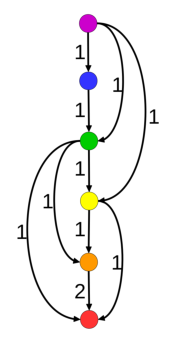
\includegraphics[width=.3\textwidth]{figures/dag.pdf}
    \caption{fig:DAGwidget}
    \label{fig:DAGwidget}
  \end{subfigure} 
  \caption{The widget}%\label{fig:example}
\end{figure}

\begin{figure}
 \begin{subfigure}[b]{0.45\textwidth}
    \centering
    \includegraphics[width=.5\textwidth]{figures/NST1An.pdf}
    \caption{fig:NSTwidget1}
    \label{fig:NSTwidget1}
  \end{subfigure}
  \quad
  \begin{subfigure}[b]{0.45\textwidth}
    \centering
    \includegraphics[width=.5\textwidth]{figures/NST2An.pdf}
    \caption{fig:NSTwidget2}
    \label{fig:NSTwidget2}
  \end{subfigure} 
  \caption{two possible changes}%\label{fig:example}
\end{figure}

\begin{figure}
 \begin{subfigure}[b]{0.45\textwidth}
    \centering
    \includegraphics[width=.5\textwidth]{figures/brick1NST.pdf}
    \caption{fig:DAGwidget1}
    \label{fig:DAGwidget1}
  \end{subfigure}
  \quad
  \begin{subfigure}[b]{0.45\textwidth}
    \centering
    \includegraphics[width=.5\textwidth]{figures/brick2NST.pdf}
    \caption{fig:DAGwidget1}
    \label{fig:DAGwidget2}
  \end{subfigure} 
  \caption{their DAG compression}%\label{fig:example}
\end{figure}


These \widgets can be pilled up as shown Figure
\ref{fig:empilement}. We will denote the tree obtained by pilling up
$n$ \widgets by $T_{n}$. The \widgets in $T_{n}$ are independent from
one another: it is possible to show that $T_{n}$ is
equidistant from every tree having the DAG compression of Figure
\ref{fig:NSTempilement} where every $A_{i}$ is either the DAG piece
Figure \ref{fig:DAGwidget1} or Figure \ref{fig:DAGwidget2}. We will
denote by $\mathcal{S}_{n}$ the set of these self nested trees. There
exists no tree closer to $T_{n}$ than these ones. %reference en annexe

\begin{figure}
 \begin{subfigure}[b]{0.45\textwidth}
    \centering
    \includegraphics[width=.5\textwidth]{figures/dag_brick.pdf}
    \caption{fig:empilement}
    \label{fig:empilement}
  \end{subfigure}
  \quad
  \begin{subfigure}[b]{0.45\textwidth}
    \centering
    \includegraphics[width=.5\textwidth]{figures/dagNST.pdf}
    \caption{fig:NSTempilement}
    \label{fig:NSTempilement}
  \end{subfigure} 
  \caption{pilling up the \widgets}\label{fig:example}
\end{figure}

To summarize, $T_{n}$ has exactly $2^{n}$ different NST and each one
of this self nested trees corresponds to an assignment of $n$
variables in $\{0;1\}$. As explained before, this could correspond to
the first step of a reduction of the NST problem. In order to complete
the reduction, we have to add \constraints. Adding \constraints means
modifing $T_{n}$ in function of the instance of INDEP-SET, in order to
obtain a tree $T$ closer to the self nested trees that correspond to valid
assignments of \variables for the instance of INDEP-SET. Given an
instance $\mathcal{I}$ of INDEP-SET, we will denote
by $\mathcal{S}_{\mathcal{I}}$ the subset of $\mathcal{S}_{n}$
constituted of the trees that correspond to valid assignments of
\variables in $\mathcal{I}$.
 
Let start with the first type of \constraint: if there is an edge
between $u$ and $v$ in the graph $G=(V,E)$ of $\mathcal{I}$, the
\variables represented by $u$ and $v$ cannot be both assigned to the
value 1. Given two vertices $u$ and $v$, if there is an edge between
$u$ and $v$, we have to modify $T_{n}$ to obtain $T$ such that $T$ is
closer to all the self nested trees of $\mathcal{S}_{n}$ where at
least one of the \widgets corresponding to $u$ and $v$ was modified
into Figure \ref{fig:DAGwidget2}, than the rest of
$\mathcal{S}_{n}$. By doing this modifications the NST of $T$ will be
the trees that correspond to a valid assignment of \variables.

The goal is to add successively this modifications for every edge in
$E$, and to reduce at every step the distance to the self nested trees
of $\mathcal{S}_{\mathcal{I}}$. By doing this modifications for every
edge in $E$, we should have applied all the \constraints of the first
type of the INDEP-SET problem and we would still have to find how to
translate the second one (the fact that only $k$ \variables can take
the value 1).

It appears that the modification for one edge has to reduce equally
the distance to all the trees of $\mathcal{S}_{\mathcal{I}}$, so that
the set of nearest self nested trees of $T$ is exactly
$\mathcal{S}_{\mathcal{I}}$. Otherwise, it is not possible to prove
the implication
$\omega_{\textsc{ NST }} = f(\omega_{\textsc{ Indep-Set }}) \in
Y_{\textsc{ NST }} \Rightarrow \omega_{\textsc{ Indep-Set }} \in
Y_{\textsc{ Indep-Set }}$

Unfortunately, the only modifications we found did not respect this
property. For this reason, we were not able to finish the proof with
this method.
 
\subsection{Last approach}

Since the second approch was not conclusive, I tried to approach the
problem form the other side: instead of trying to find the \widgets,
we will this time search to adapt the concept of \constraint to the
NST problem. 

As we said before, the \constraints are generally a sort of
translation from one problem to another of the difficulties. The issue
is that we do not know precisely at this point where the difficulty
truely lies in the NST problem. 

The algorithms proposed by C. Godin, P. Ferraro and R. Azais
\cite{godin, romain} to compute the NEST and the NeST rely on the fact
that since only addition or deletion operation are made, it is
possible to operate recursively on the DAG. More precisely, both
algorithm start by doing operations on the nodes of low height, in
order to make them all self-nested and isomorphic to one another,
recuresively use the changed nodes of low height to make the ones of
higher height alos isomorphic and self-nested. This method is possible
because only one type of operations is allowed.

Let illustrate on an example why this method does not seem to be
possible in the case of the NST problem. Let us consider the tree
Figure \ref{fig:treeexample}. Its NEST is shown Figure
\ref{fig:NESTexample}, its NeST is shown Figure \ref{fig:NeSTexample}.
Its NST is also its NEST. So far it does not seem particularly
difficult, the issue is that in tree Figure
\ref{fig:extendedexample} has for NST the tree
\ref{fig:extendedexampleNST}, where the subtrees of height 2 are
isomorphic to the tree Figure \ref{fig:NeSTexample} which is not the
NST of the subtrees of heigth 2 (isomorphic to \ref{fig:treeexample}).

The previous example highlights a sort of balance between two
irreconcilable goals: to be close to the initial tree $T$, the
subtrees of small height in the NST $S$ have to be close to the trees
of small height of $T$. But to make the higher nodes self-nested and
isomorphic to one anoher, it will sometimes be necessary to add whole
subtrees of smaller height. And therefore, the subtrees of small
height in $S$ also have to be of small size. This prevents us from
using a recursion from the bottom of the DAG to the top or in the
other direction. It prevents us from knowing where to start doing the
modifications: if we start with the upper part of the DAG, we will
need to know the exact size of the smaller subtrees to be able to
choose properly which operations have to be done; if we start with the
lower part of the DAG, we will have to know how many times the small
subtrees will be completely added in order to choose a self-nested
tree of small size yet close to the initial subtrees of small height.

The tree Figure \ref{fig:constraint} (that has the DAg compression shown
Figure \ref{fig:DAGconstraint}) is simple tree that depicts perfectly
this balance: the lower rhombus in the DAG needs to be modified in
odrer to become self-netsed, as well as the upper rhombus, but the
modifications made on any of them impacts the cost of the modifcation
made on the other one. 

This tree is at distance 12 from the self nested trees represented by
their DAG Figures \ref{fig:NST22}, \ref{fig:NST23} and \ref{fig:NST32}
and at distance 14 from the self nested tree Figure
\ref{fig:NST33}. The 3 first trees are the NST of the tree Figure
\ref{fig:constraint}. It is quite easy to see the two rhombus as
\widgets and assimilate them to \variables, that can take the values 2
or 3, depending on which one of the 4 self nested tree we consider.


\begin{figure}
 \begin{subfigure}[b]{0.45\textwidth}
    \centering
    %\includegraphics[width=.5\textwidth]{figures/dag_brick.pdf}
    \caption{fig:constraint}
    \label{fig:constraint}
  \end{subfigure}
  \quad
  \begin{subfigure}[b]{0.45\textwidth}
    \centering
    %\includegraphics[width=.5\textwidth]{figures/dagNST.pdf}
    \caption{fig:DAGconstraint}
    \label{fig:DAGconstraint}
  \end{subfigure} 
  \caption{}%\label{}
\end{figure}

\begin{figure}
 \begin{subfigure}[b]{0.22\textwidth}
    \centering
    %\includegraphics[width=\textwidth]{figures/dag_brick.pdf}
    \caption{fig:NST22}
    \label{fig:NST22}
  \end{subfigure}
  \quad
  \begin{subfigure}[b]{0.22\textwidth}
    \centering
    %\includegraphics[width=\textwidth]{figures/dagNST.pdf}
    \caption{fig:NST23}
    \label{fig:NST23}
  \end{subfigure}
  \quad
  \begin{subfigure}[b]{0.22\textwidth}
    \centering
    %\includegraphics[width=\textwidth]{figures/dag_brick.pdf}
    \caption{fig:NST32}
    \label{fig:NST32}
  \end{subfigure}
  \quad
  \begin{subfigure}[b]{0.22\textwidth}
    \centering
    %\includegraphics[width=\textwidth]{figures/dagNST.pdf}
    \caption{fig:NST33}
    \label{fig:NST33}
  \end{subfigure} 
  \caption{4 possibilites of variations}%\label{fig:example}
\end{figure}

The equal distance to the 3 first self nested tree is particularly
interessant because it is very similar to the \constraint of the
INDEP-SET problem (Figure \ref{tab:constraint})! As a short reminder,
the first type of \constraint for the INDEP-SET problem is that if two
vertices $u$ and $v$ are linked by an edge in $G$, the corresponding
\variables cannot be both set to 1.

We can see Figure \ref{tab:constraint} that the assignment of
\variables that corresponds to a valid independent set for the INDEP-SET
problem, are exactly the assignments of \variables that correspond to
the NST of the tree Figure \ref{fig:constraint}

\begin{figure}[h]
 \begin{subfigure}[b]{0.45\textwidth}
    \centering
    \begin{tabular}{|c|c|c|}
      \hline 
      $u$ & $v$ & \constraint \\
      \hline
      0 & 0 & respected \\
      0 & 1 & respected \\
      1 & 0 & respected \\
      1 & 1 & violated \\
      \hline
    \end{tabular}
    \caption{\Constraint of INDEP-SET}
    \label{tab:constIND}
  \end{subfigure}
  \quad
  \begin{subfigure}[b]{0.45\textwidth}
    \centering
    \begin{tabular}{|c|c|c|c|}
      \hline 
      $u$ & $v$ & distance & \constraint\\
      \hline
      2 & 2 & 12 & respected \\
      2 & 3 & 12 & respected \\
      3 & 2 & 12 & respected \\
      3 & 3 & 14 & violated \\
      \hline
    \end{tabular}
    \caption{\Constraint of NST}
    \label{tab:constNST}
  \end{subfigure} 
  \caption{Constraints}\label{tab:constraint}
\end{figure}

% \subsection{Intuition guiding the researches}

% \begin{itemize}
% \item Approche 1: se familariser avec le problème en se restraignant à
%   un sous-ensemble et montrer que déjà là c'est dur. Risque possible:
%   se restraindre à un sous-ensemble où en fait, c'est polynomial. Ça
%   permet quand même en général de mieux comprendre son problème.
% \item Approche 2: Preuve de NP-complétude à base de \widget,
%   i.e., de structures particulières que l'on peut combiner
%   astucieusement pour exprimer les \constraint du problème
%   auquel on cherche à se réduire.
% \item Approche 3: Trouver un graphe qui paraisse particulièrement
%   difficile.
% \end{itemize}

% In this section, I illustrate the second approach, where \widgets
% are built and linked to each others through \constraints. 

% Let us begin with the proof of the reduction from 3-SAT to INDEP-SET
% \cite{polytech}. As a brief reminder:
% \begin{definition}[3-SAT]
  
% \end{definition}

% \begin{definition}[INDEP-SET]
  
% \end{definition}
% \begin{figure}

%   \centering
  
%   \caption{3SAT reduction}
%   \label{fig:3sat}
% \end{figure}

% %%%%%%%%%%%%%%%%%%%%%%%%%%%%%%%%%%%%%%%%%%%%%%%%%%%%%%%%%%%%%%%%%%%%%%%%%%%%
% \noindent\hrulefill

% In the reduction proposed by Garey and Johnson\cite{garey}, the image
% instance of INDEP-SET is built in two steps: the first one consists in
% defining triangles that correspond to each clause of the initial
% instance of 3-SAT (see Figure\ref{fig:3sat}); the second one consists
% in adding edges that link the nodes of the \widgets that are labeled
% with the negation of the same variable of 3-SAT. One way of
% interpreting this division in two steps is to consider the triangle
% \widgets as \variables that can take three different values (the
% \variable term here should not be confused with the variable of the
% 3-SAT problem). 

% These three values are the label of three nodes of the
% triangle, and the value taken by the variable is the label of the node
% taken in the set of vertices of INDEP-SET.

% The edges linking the nodes are representing
% the constraints of the first problem

% Furthermore, we can observe that generally, the construction of the
% image instance seems to be combination of two different things: a part
% that reflects only the number of variables in the instance of the
% first problem and a part reflecting the links and constraints that
% they have with one another.  For example, in the proof of the
% reduction from 3-SAT to INDEP-SET \cite{polytech}, the first part
% consists in the triangles corresponding to each clause of the initial
% instance, and the second to the edges linking the nodes such as one is
% labeled with the negation of the other. In the proof of the reduction
% from VERTEX-COVER to HAMILTONIAN-CYCLE \cite{polytech}, the first part
% consists in the 12 nodes widgets corresponding to each edge of the
% initial graph, and the second part consists in the way they are linked
% to one another to form the image graph.

% We can also observe that in the first part, a piece of the image
% instance corresponds to each variable of the initial
% instance. Moreover, this piece of the image instance is very
% restrictive and can be used in a solution only in a few (2 or 3 most
% of the time) different ways. For example in the proof of the reduction
% from VERTEX-COVER to HAMILTONIAN-CYCLE \cite{polytech}, the widgets
% can either be visited in one pass or in two.

% Furthermore the way these pieces are used is completely independant
% until the second part corresponding to the constraints between the
% variables is added.

% \subsection{Trees of height 2 without variation of the height}
% The edit distance with constraint of K.Zhang being slightly difficult
% to manipulate, we will use a far more restrictive variant in this
% section: only leaves (and not internal nodes) can be added or
% deleted. More precisely, if $u$ is an ancestor of $v$ in $T$ and
% $v \in V'_{1}$ then $u \in V'_{1}$.

% In this section we present a polynomial algorithm computing the
% nearest self-nested tree of height 2 to a tree of height 2.

% \subsection{Trees of height 2 with variation of the height}
% In this section, we present a polynomial algorithm computing the nearest
% self-nested tree to a tree of height 2.

% \subsection{Family of bricks}
% In this section, we present a family of trees that could be used as
% the first part of the reduction to represent the variables of the
% initial instance.
% \section{Validation and consequences}
\section*{Conclusion}
\addcontentsline{toc}{section}{\protect\numberline{}Conclusion}%


%\section*{Contexte du stage}
L’équipe Inria Mosaic du RDP à l’ENS de Lyon développe des modèles
mathématiques et numériques pour étudier la morphogenèse des plantes
et des animaux. Dans ce contexte elle est amenée à concevoir des
structures de données génériques et efficaces représenter
mathématiquement les formes modélisées. Pour représenter les systèmes
ramifiés des plantes par exemple, on a souvent recours à des
structures de données arborescentes. Ces dernières sont souvent très
lourdes en mémoire et peuvent entrainer des coûts algorithmiques
importants. Pour éviter cela, l’équipe a développé depuis quelques
années une méthode permettant de compresser de façon exacte ou
approchée les structures arborescentes, basée sur l’élimination des
structures redondantes. Cette méthode conduit à représenter les
structures arborescentes par des Graphes Orientés Acycliques (DAGs). On
peut montrer que les arborescences qui se compressent sous forme de
DAGs linéaires (DAGs hamiltoniens) ont les meilleurs taux de
compression. Ces arborescences sont dites “linéaires”.  Pour
compresser une arborescence quelconque, tout en tolérant une perte
d’information, il est donc envisageable de chercher l’arborescence
linéaire la plus proche d’une arborescence donnée et de compresser
cette dernière. Ceci peut s’exprimer formellement comme un problème
d’optimisation.

\section*{Expression formelle du problème d'optimistation}
Notons $\mathcal{T}$ l'ensemble des arbres non ordonnés (c'est-à-dire
que l'on ne considère pas d'ordre sur les fils d'un noeud).
Nous noterons par la suite $T[v]$ le sous-arbre de $T$ ayant $v$ pour racine.

Considérons la relation d'équivalence $\equiv$ sur $\mathcal{T}$
définie par $T_1 \equiv T_2$ si et seulement si $T_1$ et $T_2$ sont
isomorphes. Plus généralement, nous dirons que deux sommets $v_1$ et
$v_2$, de $T_1$ et $T_2$ respectivement, sont équivalents si les
sous-arbres $T_1[v_1]$ et $T_2[v_2]$ sont isomorphes. Nous noterons
$C(v)$ la classe d'équivalence de $v$.

Pour $T = (V,E) \in \mathcal{T}$, posons
$\mathcal{Q}(T) = (V_{\mathcal{Q}}, T_{\mathcal{Q}})$ le graphe obtenu
en quotientant les sommets de $T$ par la relation
$\equiv$. Concrêtement, $V_{\mathcal{Q}} = \{ C(v) | v \in V \}$ et
$E_{\mathcal{Q}} = \{ (C(u), C(v)) | (u,v) \in T \}$. Définissons
$\delta$ la fonction de pondération sur $\mathcal{Q}(T)$ définie par
$$\delta(C(u), C(v)) = \#\{ v' \in Fils(u) | C(v) = C(v')\}$$.

La figure \ref{fig:exemple} (tirée de \cite{godin}) représente un
arbre (à gauche) et son graphe quotient (à droite). Les sommets
équivalents sont représentés d'une même couleur.

\begin {figure} [h]
  \centering
  \subfloat{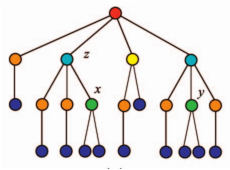
\includegraphics[width=.3\textwidth]{figures/fig1.pdf}}
  \subfloat{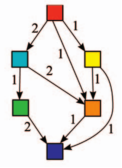
\includegraphics[width=.16\textwidth]{figures/fig2.pdf}}
  \caption{Exemple de graphe quotient}
  \label{fig:exemple}
\end{figure}

Pour tout $T \in \mathcal{T}$, $\mathcal{Q}(T)$ est un \emph{DAG} (un
graphe sans cycle orienté). De plus, pour tout \emph{DAG} $Q$, il
existe un unique $T \in \mathcal{T}$ tel que $\mathcal{Q}(T) =
Q$ \cite{godin}.

L'avantage de la représentation d'un arbre $T$ par son graphe quotient
$\mathcal{Q}(T)$ tient au fait que $\mathcal{Q}(T)$ est une
représentation compréssée. Par exemple, si une grandeur $f$ est
définie inductivement sur $\mathcal{T}$, il est possible de calculer
$f(T)$ à partir de $\mathcal{Q}(T)$, évitant ainsi d'effectuer de
nombreuses fois le même calcul sur des sous-arbres équivalents.

Les arbres dont le graphe quotient est un \emph{DAG} linéaire sont
appelés ``\emph{auto-emboîtés}''. Nous noterons $\mathcal{S}$
l'ensemble de ces arbres.

Considérons $D$ la distance d'édition sur $\mathcal{T}^{2}$ \cite{zhang}.

\section*{Attendus}
Déterminer si le problème NST défini par \\
\\
\textsc{Entrée}: $T = (V,E) \in \mathcal{T}$ \\
\textsc{Sortie}: $NST(T) := argmin_{S \in \mathcal{S}} D(T,S)$,  l'arbre auto-emboîté
le plus proche de $T$ (au sens de D).\\
\\
est NP-Complet.

% \clearpage

% \section*{Problème de décison associé}

% Il est plus facile de travailler sur le problème de décision
% naturellement associé. \\
% \textsc{Entrée}: $T = (V,E) \in \mathcal{T}$, $k \in \mathbb{N}$ \\
% \textsc{Sortie}: Oui si et seulement si il existe $S \in
% \mathcal{S}$ auto-emboîté tel que $D(T,S) \leq k$.\\
% On notera que les deux problèmes sont de difficultés équivalentes: il
% est possible de trouver la solution du problème d'optimisation à
% partir du problème de décision en temps polynomial. Il suffit pour
% cela de résolvoudre ce dernier de multiples fois en réalisant une
% dichotomie sur $k$.

% \section*{Problèmes NP-Complets}

\subsection*{Quelques définitions}
\begin{description}
\item[Problème] un problème est un langage $\mathcal{L}$ (décrit dans
  la rubrique \textsc{Entrée}), partitioné en deux sous-ensembles (la
  partition est décrite dans la rubrique \textsc{Sortie}, l'un des
  deux sous-ensembles correspond au ``oui'', l'autre au ``non'').
\item[Instance] une instance d'un problème est un élément du langage.
\item[Problème décidé par un machine de Turing] problème pour lequel il
  existe une machine de Turing renvoyant la bonne réponse en un temps
  fini pour toutes les instances.
\item[Problème accepté par un machine de Turing] problème pour lequel
  il existe une machine de Turing renvoyant oui en un temps fini pour
  les instances positives.
\item[P] est la classe des langages décidés par une machine
  de Turing déterministe en temps polynomial.
\item[NP] est la classe des langages accéptés par une machine
  de Turing non-déterministe en temps polynomial. Informellement: il
  est possible de vérifier en temps polynomial si une solution est
  valide.
\item[Réduction polynomiale] de $L_{1}$ vers $L_{2}$ est une fonction
  $f$, calculable en temps polynomial, telle que pour toute instance
  $w$ de
  $L_{1}$, $w \in L_{1} \equiv f(w) \in L_{2}$.\\
  On note alors $L_{1} \propto L_{2}$. Informellement, si l'on sait
  résoudre $L_{2}$ en temps polynomial, on sait alors résoudre $L_{1}$
  en temps polynomial, $L_{2}$ est donc au moins aussi dur que
  $L_{1}$.
\item[NP-difficile] un langage $L$ est NP-difficile si tout problème de NP
  se réduit à $L$.
\item[NP-complet] un langage est NP-complet si il est NP-difficile et
  lui-même dans la classe NP.
\end{description}

\subsection*{SAT}
\begin{itemize}
\item Problème SAT général: \\
  \textsc{Entrée}: $\phi$ une formule logique. \\
  \textsc{Sortie}: Oui si et seulement si il existe une valuation $\nu$
  telle que $\nu \models \phi$.\\
\item 3-SAT:\\
  \textsc{Entrée}: $\phi$ une formule logique sous forme 3-CNF. \\
  \textsc{Sortie}: Oui si et seulement si il existe une valuation $\nu$
  telle que $\nu \models \phi$.\\
\item NAESAT: \\
  \textsc{Entrée}: $\phi$ une formule logique sous forme CNF. \\
  \textsc{Sortie}: Oui si et seulement si il existe une valuation
  $\nu$ telle que chaque clauses contiennent au moins un littéral vrai
  et un littéral faux.\\
\item MAX-2-SAT: \\
  \textsc{Entrée}: $\phi$ une formule logique sous forme 2-CNF, $k \in
  \mathbb{N}$. \\
  \textsc{Sortie}: Oui si et seulement si il existe une valuation $\nu$
  rendant $k$ clauses de $\phi$ vraies.\\
\end{itemize}


\subsection*{INDEP-SET}
\begin{itemize}
\item INDEP-SET: \\
  \textsc{Entrée}: $G = (V, E)$ un graphe non orienté, $k\in \mathbb{N}$. \\
  \textsc{Sortie}: Oui si et seulement si il existe $S \subseteq V$ de
  taille $k$ tel que $\forall (u,v) \in S^{2}, (u,v) \notin E$.\\
\item CLIQUE: \\
  \textsc{Entrée}: $G = (V, E)$ un graphe non orienté, $k\in \mathbb{N}$. \\
  \textsc{Sortie}: Oui si et seulement si il existe une clique de taille
  $k$.\\
\end{itemize}

\subsection*{VERTEX-COVER}
\begin{itemize}
\item VERTEX-COVER: \\
  \textsc{Entrée}: $G = (V, E)$ un graphe non orienté, $k\in \mathbb{N}$. \\
  \textsc{Sortie}: Oui si et seulement si il existe $V' \subseteq V$ de
  taille $k$ tel que pour toute arête $(u,v) \in E$, $u \in V '$ ou $v \in
  V'$.\\
\item EXACT-COVER: \\
  \textsc{Entrée}: $X$ un ensemble quelconque, $\mathcal{F} \subset
  \mathcal{P}(X)$. \\
  \textsc{Sortie}: Oui si et seulement si il existe
  $\mathcal{S} \subseteq \mathcal{F}$ de taille k, tel que pour tout
  $x \in X$, il existe un unique $S \in \mathcal{S}$ tel que $x \in S$. \\
\item SUBSET-SUM: \\
  \textsc{Entrée}: $(a_{i})_{1 \leq i \leq n}$ un ensemble fini
  d'entiers, $k \in \mathbb{N}$. \\
  \textsc{Sortie}: Oui si et seulement si il existe
  $I \subset \llbracket 1;n \rrbracket$ tel que
  $\sum_{i \in I} a_{i} = k$. \\
\item PARTITION: \\
  \textsc{Entrée}: $(a_{i})_{1 \leq i \leq n}$ un ensemble fini d'entiers. \\
  \textsc{Sortie}: Oui si et seulement si il existe
  $I \subset \llbracket 1;n \rrbracket$ tel que
  $\sum_{i \in I} a_{i} = \sum_{i\notin I} a_{i}$. \\
\item 0-CYCLE: \\
  \textsc{Entrée}: $G = (V, E)$ un graphe pondéré. \\
  \textsc{Sortie}: Oui si et seulement si il existe un cycle $C$ de
  poids nul. \\
\item BIN-PACKING: \\
  \textsc{Entrée}: $(a_{i})_{1 \leq i \leq n}$ un ensemble fini
  d'entiers (taille des objets), une infinité de boîtes de taille $C \in
  \mathbb{N}$, $k \in \mathbb{N}$. \\
  \textsc{Sortie}: Oui si et seulement si il est possible de ranger
  l'intégralité des objets dans moins de $k$ boîtes.\\
\item KNAPSACK: \\
  \textsc{Entrée}: un ensemble fini d'objets, de poids
  $(w_{i})_{1 \leq i \leq n}$ et de valeur $(v_{i})_{1 \leq i \leq
    n}$, deux entiers $W$ et $V$. \\
  \textsc{Sortie}: Oui si et seulement si il existe
  $(x_{i})_{1 \leq i \leq n} \in \{0, 1\}^{n}$
  tel que $\sum_{i = 1}^{n} x_{i}w_{i} \leq W$ et $\sum_{i
    = 1}^{n} x_{i}v_{i} \geq V$.\\
\end{itemize}

\subsection*{Circuits et chemins}
\begin{itemize}
\item HAMILTONIAN-PATH:
  \textsc{Entrée}: $G = (V, E)$ un graphe. \\
  \textsc{Sortie}: Oui si et seulement si $G$ admet un cycle hamiltonien.\\
\item TSP: \\
  \textsc{Entrée}: $G = (V, E)$ un graphe, $k\in \mathbb{N}$. \\
  \textsc{Sortie}: Oui si et seulement si il existe un cycle
  hamiltonien de poids inférieur à $k$.\\

\end{itemize}

\subsection*{Quelques autres}
\begin{itemize}
\item CHROMATIC-NUMBER: \\
  \textsc{Entrée}: $G = (V, E)$ un graphe non orienté, $k\in \mathbb{N}$. \\
  \textsc{Sortie}: Oui si et seulement si il existe $k$-coloration de $G$.\\

\item MAX-CUT: \\
  \textsc{Entrée}: $G = (V, E)$ un graphe non orienté pondéré, $k\in \mathbb{N}$. \\
  \textsc{Sortie}: Oui si et seulement si il existe une coupe
  $C \subset V$ de poids $w(C, \complement_{V}C) \geq k$.\\
\end{itemize}


% \clearpage

% \section{Preuve de l'apartenance à NP}

Soient $T \in \mathcal{T}$ et $S \in \mathcal{S}$, $k \in \mathbb{N}$.
Il est possible de calculer la distance d'édition contrainte $D(T,S)$
en temps polynomial (\cite{zhang}).

% \section{Lemmes et remarques intermédiaires}

\subsection{Arbre de hauteur 2, sans modification de hauteur}

Nous nous intéressons ici aux arbres de hauteur 2 dont les feuilles
sont toutes de profondeur 2. Notons $\mathcal{T}_{2}$ l'ensemble de
ces arbres.

\begin{center}
\begin{forest}
  for tree={
    circle,
    draw
  }
  [
    [
      []
      []
      []
    ]
    [
      []
    ]
    [
      []
      []
    ]
  ]
\end{forest}
\end{center}
%Insérer un dessin

Nous imposons plusieurs contraintes à la distance d'édition:
premièrement, nous n'autorisons pas l'ajout ou la suppression de nœuds
internes; de plus, nous imposons aux arbres comparés d'avoir la même
hauteur.

Soit $T \in \mathcal{T}_{2}$. Numérotons
$(u_{i}^{(T)})_{1 \leqslant i \leqslant N}$ les noeuds de profondeur 1
de $T$. Notons $(n_{i})_{1 \leqslant i \leqslant N}$ leur
nombre de fils respectifs. \\
Soit $S = NST(T)$, nous noterons
$(u_{i}^{(S)})_{1 \leqslant i \leqslant N}$ les images des
$(u_{i}^{(T)})_{1 \leqslant i \leqslant N}$ par le mapping. \\
Notons pour $k \in \mathbb{N}$,
$I_{k} = \{ i \in \llbracket 1;N \rrbracket | h(u_{i}^{(S)}) = k\}$
les indices des nœuds de profondeur 1 dont le mapping est de hauteur $k$.\\

\begin{rem}
\label{rem1}
$S$ étant de hauteur 2, dans cette section, $(I_{0}, I_{1})$ forme une
partition de $\llbracket 1;N \rrbracket$.
\end{rem}

\begin{lem}
  \label{lem1}
  Notons $\tilde{n}$ le nombre de fils des sous arbres de hauteur 1
  dans $S$.\\
  Nous avons la formule suivante:
  $$D(T,S) = \sum_{i \in I_{0}} n_{i} + \sum_{i \in I_{1}} |n_{i} - \tilde{n}|$$
  
  \begin{proof}
    Pour obtenir $S$ à partir de $T$, il faut supprimer les fils de
    $u_{i}^{(T)}$ pour tout $i \in I_{0}$, soit $\sum_{i \in I_{0}} n_{i}$
    nœuds au total. De plus pour chaque $i \in I_{1}$,
    \begin{itemize}
    \item si $n_{i} > \tilde{n}$, il faut supprimer
      $n_{i} - \tilde{n}$ fils de $u_{i}^{(T)}$,
    \item si $n_{i} < \tilde{n}$, il faut en ajouter
      $\tilde{n} - n_{i}$, 
    \end{itemize}
    soit un total de $\sum_{i \in I_{1}} |n_{i} - \tilde{n}|$ ajout
    ou suppression. D'où le résultat.
  \end{proof}
\end{lem}

\begin{lem}
  \label{lem2}
  Soit $(I_{0}, I_{1})$ une partition de $\llbracket 1;N \rrbracket$
  fixée (non nécessairement optimale).\\
  $\sum_{i \in I_{0}} n_{i} + \sum_{i \in I_{1}} |n_{i} - \tilde{n}|$
  atteint son minimum en $\tilde{n}$ l'une des médianes des
  $(n_{i})_{i \in I_{1}}$.
\end{lem}

\begin{rem}
  \label{rem2}
  Dans le cadre de notre étude, $\tilde{n}$ doit prendre une valeur
  entière. Aussi, si $I_{1}$ est de cardinal pair et que les deux
  valeurs médianes sont distinctes, nous fixerons $\tilde{n}$ à la
  plus grande des deux valeurs. Ce choix ne modifie en effet pas la
  distance.
\end{rem}

\begin{lem}
  \label{lem3}
  Soit $(I_{0}, I_{1})$ une partition de $\llbracket 1;N \rrbracket$
  fixée (non nécessairement optimale).\\
  Soit $\tilde{n}$ la médiane des $(n_{i})_{i \in I_{1}}$ .
  Soit $S$ l'arbre auto-emboîté défini par $(I_{0}, I_{1})$ et $\overline{n}$.\\
  Supposons qu'il existe $i \in I_{0}$ tel que $n_{i} \geqslant
  \tilde{n}$.
  Soit $S'$ l'arbre auto-emboîté défini par $(I_{0} \setminus \{i\},
  I_{1} \cup \{i\})$ et $\tilde{n}$.\\
  On a l'égalité suivante: $$D(T,S) \geqslant D(T,S')$$
  \begin{proof}
    Calculons la différence:
    \begin{center}
      $
      \begin{array}{rcl}
        D(T,S) - D(T,S') &=& \left( \sum_{k \in I_{0}} n_{k} + \sum_{k \in
                            I_{1}} |n_{k} - \tilde{n}| \right) -\left( \sum_{k \in
                            I_{0}\setminus \{k\}} n_{k} + \sum_{k \in
                            I_{1} \cup \{k\}} |n_{k} - \tilde{n}| \right)\\
                        &=& n_{i} - |n_{i} - \tilde{n}|\\
                        & \geqslant & 0
      \end{array}
      $
    \end{center}
    
  \end{proof}
\end{lem}

\begin{lem}
  \label{lem4}
  Soit $(I_{0}, I_{1})$ une partition de $\llbracket 1;N \rrbracket$
  fixée (non nécessairement optimale).\\
  Soit $\tilde{n}$ la médiane des $(n_{i})_{i \in I_{1}}$.
  Soit $S$ l'arbre auto-emboîté défini par $(I_{0}, I_{1})$ et $\tilde{n}$.\\
  Soit $j = argmin_{k \in I_{1}}n_{k}$.  Supposons qu'il existe
  $i \in I_{0}$ tel que $n_{j} < n_{i} < \tilde{n}$.\\
  Posons $I_{0}' = (I_{0} \setminus \{i\}) \cup \{j\}$ et
  $I_{1}' = (I_{1} \setminus \{j\}) \cup \{i\}$. Soit
  $\tilde{n}'$ la médiane des $(n_{i})_{i \in I_{1}'}$.\\
  Soit $S'$ l'arbre auto-emboîté défini par $(I_{0}', I_{1}')$ et
  $\tilde{n}'$. On a l'inégalité suivante:
  $$D(T,S) \geqslant D(T,S')$$
  \begin{proof}
    Comme $n_{j} < n_{i} < \tilde{n}$, on a $\tilde{n} = \tilde{n}'$.
    On a donc 
    \begin{center}
      $
      \begin{array}{rcl}
        D(T,S) - D(T,S') &=& \left( \sum_{k \in I_{0}} n_{k} + \sum_{k \in
                            I_{1}} |n_{k} - \tilde{n}| \right) -\left( \sum_{k \in
                            I_{0}'} n_{k} + \sum_{k \in
                            I_{1}'} |n_{k} - \tilde{n}| \right)\\
                        &=& n_{i} - n_{j} + |n_{j} - \tilde{n}| -|n_{i} - \tilde{n}|\\
                        & \geqslant & 0
      \end{array}
      $
    \end{center}
    car $n_{j} < n_{i} < \tilde{n}$.
  \end{proof}
\end{lem}

\begin{algorithm}
\label{algo1}
\caption{Compute the NST of a tree of height 2}
\begin{algorithmic} 
\REQUIRE $(n_{i})_{1 \leqslant i \leqslant N}$ in ascending order.
\STATE $M_{min} \leftarrow 0$
\STATE $\tilde{n} \leftarrow n_{\left\lceil \frac{N}{2} \right\rceil}$ 
\STATE $current\_dist \leftarrow \sum_{i=1}^{N} |n_{i} - \overline{n}|$
\STATE $dist_{min} \leftarrow current\_dist$
\FOR{$k \in \llbracket 1;N \rrbracket$}
\STATE $\tilde{n} \leftarrow n_{\left\lceil \frac{N+k}{2} \right\rceil}$ 
\STATE $current\_dist \leftarrow \sum_{i = 1}^{k} n_{i} + \sum_{i=
  k+1}^{N} |n_{i} - \tilde{n}|$
\IF{$current\_dist < dist_{min}$}
\STATE $dist_{min} \leftarrow current\_dist$
\STATE $M_{min} \leftarrow k$
\ENDIF
\ENDFOR
\RETURN $(dist, M_{min}, n_{\left\lceil \frac{N + M_{min}}{2} \right\rceil})$ 
\end{algorithmic}
\end{algorithm}

\begin{thm}
  \label{thm1}
  L'algorithme \ref{algo1} calcule l'arbre auto-emboité le plus proche de $T \in
  \mathcal{T}_{2}$ donné en entrée, ainsi que la distance les
  séparant. De plus, il s'éxécute en temps polynomial en $N$.
  \begin{proof}
    Soit $T \in \mathcal{T}_{2}$. Soit $(I_{0}, I_{1})$
    optimals. D'après les lemmes \ref{lem3} et \ref{lem4}, pour tout
    $i \in I_{0}$, pour tout $j \in I_{1}$, $n_{i} < n_{j}$.\\
    Donc $(I_{0},I_{1})$ sépare les
    $(n_{i})_{i \in \llbracket 1;N \rrbracket}$ en deux parties, l'une
    dont les élements sont supérieurs à $M \in \mathbb{N}$, l'autre
    dans laquelle ils sont inférieurs à $M$. Par conséquent, en
    ordonnant les $(n_{i})_{i \in \llbracket 1;N \rrbracket}$ par
    ordre croissant et en augmentant $M$ progressivement, la partition
    optimale sera atteinte.
  \end{proof}
\end{thm}

\subsection{Arbre de hauteur 2, avec modification de hauteur}

Nous enlevons à présent la contrainte de non-variation de la hauteur
des sous arbres conservés.

\begin{lem}
  \label{lem5}
  Soit $T \in \mathcal{T}_{2}$. Notons $S = NST(T)$. \\
  Tout nœud $u \in S$ de profondeur non nulle (autre que la racine),
  posséde au plus un fils de hauteur non nulle.

  \begin{proof}
    Raisonnons par l'absurde. Supposons qu'il existe un nœud $u$ de
    profondeur non nulle possédant au moins deux fils $v_{1}$ et
    $v_{2}$ de hauteur non nulle. Quitte à inverser $v_{1}$ et
    $v_{2}$, on peut supposer que $h(v_{1}) \geqslant h(v_{2})$.

    Considérons l'arbre $S'$ obtenu depuis $S$ en réduisant à une
    feuille un sous arbre isomorphe à $S[v_{2}]$, dans
    chaque sous-arbres isomorphes à $S[u]$.

    \begin{center}
      \begin{forest}
        for tree={
          circle,
          draw
        }        
        [
          [
            [$u$
              [$v_{1}$
                [
                  []
                ]
              ]
              [$v_{2}$
                []
              ]
              []
            ]
            []
            []
          ]
          [
            [
              [
                []
              ]
            ]
            [
              []
            ]
            []
          ]
          [
            [
              []
            ]
          ]
        ]
      \end{forest}
      \quad
            \begin{forest}
        for tree={
          circle,
          draw
        }        
        [
          [
            [$u$
              [$v_{1}$
                [
                  []
                ]
              ]
              [$v_{2}$]
              []
            ]
            []
            []
          ]
          [
            [
              [
                []
              ]
            ]
            []
            []
          ]
          [
            [
              []
            ]
          ]
        ]
      \end{forest}

    \end{center}
    $S'$ est alors auto-emboîté et son nombre de sommet de profondeur
    supérieure à 2 est strictement inférieur à celui dans $S$. Or tout
    les nœuds de profondeur supérieure à 2 n'appartiennent pas à $T$
    qui est de hauteur 2 (découle de la propriété de non
    ajout/suppression de nœuds internes). 

    Par conséquent, $D(T,S') < D(T,S)$ ce qui est absurde.
  \end{proof}
\end{lem}

\begin{lem}
  \label{lem6}
  Soit $T \in \mathcal{T}_{2}$. Notons $S = NST(T)$. \\
  S'il existe un nœud $u \in S$ de prondeur 1 et de hauteur $k$, avec
  $k \geqslant 2$, alors il existe un nœud $v \in S$ de profondeur 1
  et de hauteur $k-1$.
  
  \begin{proof}
    Raisonnons par l'absurde. Supposons qu'il existe un nœud
    $u_{1} \in S$ de profondeur 1 et de hauteur $k$, avec $k \geqslant 2$, mais
    aucun nœud $v \in S$ de profondeur 1 et de hauteur $k-1$.

    $u_{1}$ étant de hauteur $k \geqslant 2$, $u_{1}$ possède un fils de hauteur non
    nulle. D'après le lemme précédent, ce dernier est unique, nommons
    le $u_{2}$. Deux cas de figures sont alors possibles:
    \begin{enumerate}
    \item $u_{2}$ est de hauteur $k - 1 = 1$. Notons alors $u_{3}$ l'un de
      ses fils.
    \item $u_{2}$ est de hauteur $k - 1 \geqslant 2$. Par le même raisonnement
      que pécédemment, notons $u_{3}$ l'unique fils de $u_{2}$ de hauteur non-nulle. 
    \end{enumerate}

    Considérons $S'$ l'arbre obtenu depuis $S$ en remplacant les
    sous-arbres isomorphes à $S[u_{2}]$ par $S[u_{3}]$. %insérer un dessin
    
    \begin{center}
      \begin{forest}
        for tree={
          circle,
          draw
        }        
        [
          [
            [
              [
                [
                  [
                   []
                  ]
                ]
                []
              ]
              []
              []
            ]
          ]
          [$u_{1}$
            [$u_{2}$
              [$u_{3}$
                [
                  []
                ]
              ]
              []
            ]
            []
            []
          ]
          [
            [
              []
            ]
          ]
          [
            []
          ]
          [
            []
          ]
        ]
      \end{forest}
      \quad
      \begin{forest}
        for tree={
          circle,
          draw
        }        
        [
          [
            [
              [
                [
                 []
                ]
              ]
              []
            ]
          ]
          [$u_{1}$
            [$u_{3}$
              [
                []
              ]
            ]
            []
          ]
          [
            [
              []
            ]
          ]
          [
            []
          ]
          [
            []
          ]
        ]
      \end{forest}
    \end{center}
    $S'$ est alors auto-emboîté car $S$ ne contenait pas de nœud de
    profondeur 1 et de hauteur $k - 1$. 

    De plus le nombre de sommets de $S'$ de profondeur supérieure à 3
    est strictement inférieur à celui dans $S$. Or tout les nœuds de
    profondeur supérieure à 3 n'appartiennent pas à $T$ qui est de
    hauteur 2 (découle de la propriété de non ajout/suppression de
    nœuds internes). De plus, le nombre de nœuds de profondeur
    inférieur à 2 est inchangé car aucun des nœuds de $S$ de profondeur 1
    n'est de hauteur $k - 1$ et donc n'est remplacé par $S[u_{3}]$.

    Par conséquent, $D(T,S') < D(T,S)$ ce qui est absurde.
  
  \end{proof}
\end{lem}

\begin{prop}
  \label{prop1}
  Soit $T \in \mathcal{T}_{2}$. Soit $S = NST(T)$. \\
  En notant $n_{min} = min_{1 \leqslant i \leqslant N} n_{i}$,
  nous avons la formule suivante:
  $$h(S) \leqslant \frac{3}{2} +\sqrt{\frac{9}{4} + 4 \left( \left(\sum_{i \in
          \llbracket 1;N \rrbracket}n_{i} \right) - N n_{min} \right)} $$ 
  c'est-à-dire
  $$h(S) \leqslant \frac{3}{2} +\sqrt{\frac{9}{4} + 4 \left( |T| - N
      (n_{min} + 1) -1 \right)} $$  
  \begin{proof}
    $T$ est de hauteur 2. \\
    Pour atteindre une hauteur $h(S)$, il faut que pour tout
    $k \in \llbracket 2;h(S)-1 \rrbracket$, il existe dans $S$ un nœud
    $u_{i}^{S}$ de profondeur 1 et de hauteur $k$.  Il faut donc
    ajouter au moins $\sum_{k=1}^{h(S) - 2}k =
    \frac{(h(S) -2)(h(S)-1)}{2}$ à $T$ pour obtenir $S$.\\
    Considérons l'arbre $S'$ obtenu depuis $T$ en supprimant des
    feuilles jusqu'à ce que pour tout $i$, $n_{i}^{S} = n_{min}$. $S'$ est
    un arbre auto-emboîté dont la distance à $T$ est
    $$D(T,S') = \left(\sum_{i \in \llbracket 1;N \rrbracket}n_{i} \right) - N n_{min} = |T| - N (n_{min} + 1) - 1$$
    On a donc
    $D(T,S') \geqslant D(T,S) \geqslant \frac{(h(S)
      -2)(h(S)-1)}{2}$.
    En résolvant cette équation du second degré en $h(S)$, nous obtenons
    $$h(S) \leqslant \frac{3}{2} +\sqrt{\frac{9}{4} + 4 D(T,S')}$$
  \end{proof}
\end{prop}

\subsection{Work in progress}
\begin{lem}
  \label{lem7}
  Soit $T \in \mathcal{T}_{2}$. Soit $S = NST(T)$. Notons pour tout
  $k \in \mathbb{N}$, $I_{k}$ l'ensemble des indices
  $i \in \llbracket 1;N \rrbracket$ pour lesquels $u_{i}^{(S)}$ est de
  hauteur $k$. \\
  Notons $H = h(S)$. Notons pour tout
  $k \in \llbracket 1;H \rrbracket$, $\tilde{n}^{k}$ le
  nombre de fils des nœuds de prondeur 1 et de hauteur $k$ dans $S$.\\
  On a la formule suivante :
  $$ D(S,T) = \sum_{i \in I_{0}} n_{i} + \sum_{k = 1}^{H} \left(
    \sum_{i \in I_{k}} |n_{i} - \tilde{n}^{k}| + |I_{k}|\sum_{l =
      1}^{k-1}(\tilde{n}^{l}) \right)$$
  \begin{proof}
    Pour obtenir $S$ à partir de $T$, il faut supprimer les fils de
    $u_{i}^{(T)}$ pour tout $i \in I_{0}$, soit $\sum_{i \in I_{0}} n_{i}$
    nœuds au total. De plus pour chaque $i \in I_{k}$,
    \begin{itemize}
    \item si $n_{i} > \tilde{n}^{k}$, il faut supprimer
      $n_{i} - \tilde{n}^{k}$ fils de $u_{i}^{(T)}$,
    \item si $n_{i} < \tilde{n}^{k}$, il faut en ajouter
      $\tilde{n}^{k} - n_{i}$. 
    \end{itemize}
    L'un des fils de $u_{i}^{S}$ est de hauteur $k-1$, il faut donc
    ajouter de plus $\sum_{l = 1}^{k-1}(\tilde{n}^{l})$ nœuds sous
    celui-ci. En effet, d'après le lemme \ref{lem5}, les sous-arbres
    de hauteur $k \geqslant 1$ de $S$ contiennent
    $\tilde{n}^{k-1} + \left| S^{(k-1)} \right|$ nœuds, où
    $ \left| S^{(k-1)} \right|$ est le nombre de nœuds des sous arbres
    de $S$
    de hauteur $k-1$. On montre alors aisément par récurrence que
    $\left| S^{(k-1)} \right| = 1 + \sum_{l =
      1}^{k-1}(\tilde{n}^{l})$.\\
    Soit un total de
    $\sum_{i \in I_{1}} |n_{i} - \tilde{n}| + |I_{k}|\sum_{l =
      1}^{k-1}(\tilde{n}^{l})$ ajout ou suppression. D'où le résultat.
 
  \end{proof}
\end{lem}

\begin{rem}
  \label{rem3}
   $$ D(S,T) = \sum_{i \in I_{0}} n_{i} + \sum_{k = 1}^{H} \left(
    \sum_{i \in I_{k}} |n_{i} - \tilde{n}^{k}| + \tilde{n}^{k}\sum_{l =
      k+1}^{H}(|I_{l}|) \right)$$
\end{rem}

\begin{lem}
  \label{lem8}
  Soit $T \in \mathcal{T}_{2}$. Soit $S = NST(T)$.  Soient
  $(I_{k})_{0 \leqslant k \leqslant h(S)}$ et
  $(\tilde{n}^{k})_{1 \leqslant k \leqslant h(S)}$ les suites
  associées.\\
  Pour tout $k \in \llbracket 1;H-1 \rrbracket$, $$|I_{k}| > \sum_{l=
      k+1}^{H}|I_{l}|$$
    \begin{proof}
      Supposons le contraire, soit $k \in \llbracket 1;H-1 \rrbracket$
      tel que $|I_{k}| \leqslant \sum_{l= k+1}^{H}|I_{l}|$.Posons
    $(J_{l})_{0 \leqslant \leqslant h(S)-1}$ et
    $(\tilde{m}^{\ l})_{1 \leqslant \leqslant h(S)-1}$ où
    \begin{align*}
      J_{l} =
      \begin{cases}
        I_{k} \cup I_{0} &\mbox{si } l=0\\       
        I_{l} &\mbox{si } 1 \leqslant l \leqslant k-1\\
        I_{l+1} &\mbox{sinon.}
      \end{cases}
                  \text{ et } \tilde{m}^{\ l} =
                  \begin{cases}
                    \tilde{n}^{l} &\mbox{si } 1 \leqslant l \leqslant k-1\\
                    \tilde{n}^{l+1} &\mbox{sinon.}
                  \end{cases}
    \end{align*}
    Notons $S'$ l'arbre auto-emboîté associé aux
    $(J_{l})_{0 \leqslant \leqslant h(S)-1}$ et
    $(\tilde{m}^{l})_{0 \leqslant \leqslant h(S)-1}$.
    \begin{center}
      $$
      \begin{array}{rcl}
        D(T,S) - D(T,S') &=& \left( \sum_{i \in I_{k}}
                             |n_{i}-\tilde{n}^{k}|+ |I_{k}|
                             \sum_{l=1}^{k-1} \tilde{n}^{l} + |\tilde{n}^{k}|
                             \sum_{l=k+1}^{h(S)} |I_{l}| \right) -
                             \sum_{i \in I_{k}} n_{i}  \\

                         &=& \sum_{i \in I_{k}} \left(|n_{i} -
                             \tilde{n}^{k}| - n_{i} +\left( \sum_{l=1}^{k-1}
                             \tilde{n}^{l} \right)\right) +
                             \tilde{n}^{k}\sum_{l=k+1}^{H} |I_{l}| \\
                         &\geqslant& \sum_{i \in I_{k}} \left(|n_{i} -
                                     \tilde{n}^{k}| + (\tilde{n}^{k}
                                     -n_{i}) + \left( \sum_{l=1}^{k-1}
                                     \tilde{n}^{l} \right) \right) \\
                         &>& \sum_{i \in I_{k}} \left(|n_{i} -
                             \tilde{n}^{k}| + (\tilde{n}^{k}
                             -n_{i}) \right)\\
                         &>& 0
      \end{array}
      $$
    \end{center}
    Donc $D(T,S) > D(T,S')$ ce qui est absurde car $S'$ est auto-emboîté.
  \end{proof}
\end{lem}

\begin{cor}
  \label{cor1}
  On a pour tout $k \in \llbracket 1;H \rrbracket$, $|I_{k}| \geqslant 2^{H-k}$.
  De plus, en notant $N$ le nombre de nœuds de $T$ de profondeur 1, on a 
  $$h(S) \leqslant \left\lfloor \log_{2}(N+1) \right\rfloor$$
  \begin{proof}
    En notant $H = h(S)$, on a
    \begin{center}
      $$
      \begin{array}{rcl}
        |I_{k}| &\geqslant& \sum_{l=k+1}^{H} |I_{l}| + 1\\
                &\geqslant& |I_{k+1}| + \sum_{l=k+2}^{H} |I_{l}| + 1 \\
                &\geqslant& 2(\sum_{l=k+2}^{H} |I_{l}| + 1) \\
                &\geqslant& 2^{H-k-1}(I_{H} +1)\\
                &\geqslant& 2^{H-k}\\
      \end{array}
      $$
    \end{center}
    Donc $N
    \geqslant \sum_{k=1}^{H} |I_{k}| \geqslant \sum_{k=1}^{H} 2^{H-k}
    \geqslant 2^{H} -1$. \\
    Donc $H \leqslant \left\lfloor \log_{2}(N+1) \right\rfloor$
      \end{proof}
\end{cor}

\begin{lem}
  \label{lem9}
  Soit $T \in \mathcal{T}_{2}$. Soit $S = NST(T)$.  Soient
  $(I_{k})_{0 \leqslant k \leqslant h(S)}$ et
  $(\tilde{n}^{k})_{1 \leqslant k \leqslant h(S)}$ les suites
  associées.\\
  Pour tout $k \in \llbracket 2;H \rrbracket$, $$\tilde{n}^{k} > \sum_{l=1}^{k-1}\tilde{n}^{k}$$
    \begin{proof}
      Supposons le contraire, soit $k \in \llbracket 2;H \rrbracket$
      tel que
      $\tilde{n}^{k} \leqslant \sum_{l= 1}^{k-1} \tilde{n}^{l}$.Posons
      $(J_{l})_{0 \leqslant \leqslant h(S)-1}$ et
      $(\tilde{m}^{\ l})_{1 \leqslant \leqslant h(S)-1}$ où
    \begin{align*}
      J_{l} =
      \begin{cases}
        I_{k} \cup I_{0} &\mbox{si } l=0\\       
        I_{l} &\mbox{si } 1 \leqslant l \leqslant k-1\\
        I_{l+1} &\mbox{sinon.}
      \end{cases}
                  \text{ et } \tilde{m}^{\ l} =
                  \begin{cases}
                    \tilde{n}^{l} &\mbox{si } 1 \leqslant l \leqslant k-1\\
                    \tilde{n}^{l+1} &\mbox{sinon.}
                  \end{cases}
    \end{align*}
    Notons $S'$ l'arbre auto-emboîté associé aux
    $(J_{l})_{0 \leqslant \leqslant h(S)-1}$ et
    $(\tilde{m}^{l})_{0 \leqslant \leqslant h(S)-1}$.
    \begin{center}
      $$
      \begin{array}{rcl}
        D(T,S) - D(T,S') &=& \left( \sum_{i \in I_{k}}
                             |n_{i}-\tilde{n}^{k}|+ |I_{k}|
                             \sum_{l=1}^{k-1} \tilde{n}^{l} + |\tilde{n}^{k}|
                             \sum_{l=k+1}^{h(S)} |I_{l}| \right) -
                             \sum_{i \in I_{k}} n_{i}  \\

                         &=& \sum_{i \in I_{k}} \left(|n_{i} -
                             \tilde{n}^{k}| +\left( \sum_{l=1}^{k-1}
                             \tilde{n}^{l} \right) - n_{i} \right) +
                             \tilde{n}^{k}\sum_{l=k+1}^{H} |I_{l}| \\
                         &>& \sum_{i \in I_{k}} \left(|n_{i} -
                             \tilde{n}^{k}| +\left( \sum_{l=1}^{k-1}
                             \tilde{n}^{l} \right) - n_{i}\right)\\
                         &>& \sum_{i \in I_{k}} \left(|n_{i} -
                             \tilde{n}^{k}| + (\tilde{n}^{k} - n_{i})\right)\\                         
                         &>& 0
      \end{array}
      $$
    \end{center}
    Donc $D(T,S) > D(T,S')$ ce qui est absurde car $S'$ est auto-emboîté.
  \end{proof}
\end{lem}

\begin{cor}
  \label{cor2}
  On a pour tout $k
  \in \llbracket 1;H \rrbracket$, $\tilde{n}^{k} \geqslant
  2^{k}$. \\
  De plus, en notant $n_{max}
  = max_{i \in \llbracket 1,;N \rrbracket} n_{i}$, on a $h(S)
  \leqslant \left\lfloor \log_{2}(n_{max}+1) \right\rfloor$
  \begin{proof}
    En notant $H = h(S)$, on a 
    \begin{center}
      $$
      \begin{array}{rcl}
        \tilde{n}^{k} &\geqslant& \sum_{l=1}^{k-1} \tilde{n}^{l} + 1\\
                      &\geqslant& \tilde{n}^{k-1} + \sum_{l=1}^{k-2}
                                  \tilde{n}^{l} + 1 \\
                      &\geqslant& 2(\sum_{l=1}^{k-2} \tilde{n}^{l} + 1) \\
                      &\geqslant& 2^{k-1}(\tilde{n}^{1} +1)\\
                      &\geqslant& 2^{k}\\
      \end{array}
      $$
    \end{center}
    Donc $n_{max} \geqslant \tilde{n}^{H}
    \geqslant \sum_{k=1}^{H-1} \tilde{n}^{l} \geqslant \sum_{k=1}^{H-1} 2^{k}
    \geqslant 2^{H} -1$. \\
    Donc $H \leqslant \left\lfloor \log_{2}(n_{max}+1) \right\rfloor$
      \end{proof}
\end{cor}

\begin{lem}
  \label{lem10}
  Soit $T \in \mathcal{T}_{2}$. Soit $S = NST(T)$.  Soient
  $(I_{k})_{0 \leqslant k \leqslant h(S)}$ et
  $(\tilde{n}^{k})_{1 \leqslant k \leqslant h(S)}$ les suites
  associées.\\
  Pour tout $k \in \llbracket 1;H \rrbracket$, $\tilde{n}^{k}$
  minimise
  $\sum_{i \in I_{k}} |n_{i} - \tilde{n}^{k}| +
  \tilde{n}^{k}\sum_{l=k+1}^{h(S)}|I_{l}|$.\\ 
  $\tilde{n}^{k}$ est donc la $\left\lfloor \frac{|I_{k}|
      - \sum_{l=k+1}^{h(S)}|I_{l}|}{2} \right\rfloor$ ème plus petite
  valeur de $\{n_{i} | i \in I_{k} \}$.
\end{lem}

\begin{lem}
  \label{lem11}
  Soit $T \in \mathcal{T}_{2}$. Soit $S = NST(T)$.  Soient
  $(I_{k})_{0 \leqslant k \leqslant h(S)}$ et
  $(\tilde{n}^{k})_{1 \leqslant k \leqslant h(S)}$ les suites
  associées.\\
  Pour tout $i \in \llbracket 1;N \rrbracket$, si $\tilde{n}^{k}
  \leqslant n_{i} \leqslant \tilde{n}^{k+1}$ alors $i \in I_{k} \cup
  I_{k+1}$
  \begin{proof}
    D'après le lemme \ref{lem10}
    $(\tilde{n}^{k})_{1 \leqslant k \leqslant h(S)}$ est
    croissante. Par conséquence, $i \in \bigcup_{l \leqslant k+1}
    I_{l}$.\\
    Supposons que $i \in I_{h}$ avec $h \leqslant k-1$.
    
    Notons $S'$ l'arbre auto-emboîté associé aux
    $(J_{l})_{0 \leqslant \leqslant h(S)-1}$ et
    $(\tilde{m}^{l})_{0 \leqslant \leqslant h(S)-1}$.
    \begin{center}
      $$
      \begin{array}{rcl}
        D(T,S) - D(T,S') &=& |n_{i}-\tilde{n}^{h}| -
                             |n_{i}-\tilde{n}^{k}| + \sum_{l=1}^{h-1}
                             \tilde{n}^{l} -\sum_{l=1}^{k-1} \tilde{n}^{l}\\
                         &=& n_{i} - \tilde{n}^{h} -
                             (n_{i}-\tilde{n}^{k}) - \sum_{l=h}^{k-1}
                             \tilde{n}^{l} \\
                         &=& \tilde{n}^{k} - \tilde{n}^{h} -
                             \sum_{l=h}^{k-1} \tilde{n}^{l} \\
                         &>& \sum_{l=1}^{k-1} \tilde{n}^{l} -
                             \tilde{n}^{h} - \sum_{l=h}^{k-1} \tilde{n}^{l} \\
                         &>& \sum_{l=1}^{h-1} \tilde{n}^{l} -
                             \tilde{n}^{h}\\
                         &>&0
      \end{array}
      $$
    \end{center}
    Les inégalités ci-dessus découle du lemme \ref{lem9}. 
    On a donc $D(T,S) > D(T,S')$ ce qui est absurde car $S'$ est auto-emboîté.
  \end{proof}
\end{lem}

\begin{lem}
  \label{lem12}
  Soit $T \in \mathcal{T}_{2}$. Soit $S = NST(T)$.  Soient
  $(I_{k})_{0 \leqslant k \leqslant h(S)}$ et
  $(\tilde{n}^{k})_{1 \leqslant k \leqslant h(S)}$ les suites
  associées.\\
  Pour tout $i \in \llbracket 1;N \rrbracket$, si $\tilde{n}^{k}
  \leqslant n_{i} \leqslant \sum_{l=1}^{k+1}\tilde{n}^{l}$ alors $i \in I_{k}$
  \begin{proof}
    D'après le lemme \ref{lem11}, $i \in I_{k} cup I_{k+1}$.\\
    Supposons que $i \in I_{k+1}$.
    
    Notons $S'$ l'arbre auto-emboîté associé aux
    $(J_{l})_{0 \leqslant \leqslant h(S)-1}$ et
    $(\tilde{m}^{l})_{0 \leqslant \leqslant h(S)-1}$.
    \begin{center}
      $$
      \begin{array}{rcl}
        D(T,S) - D(T,S') &=& |n_{i}-\tilde{n}^{h}| -
                             |n_{i}-\tilde{n}^{k}| + \sum_{l=1}^{h-1}
                             \tilde{n}^{l} -\sum_{l=1}^{k-1} \tilde{n}^{l}\\
                         &=& n_{i} - \tilde{n}^{h} -
                             (n_{i}-\tilde{n}^{k}) - \sum_{l=h}^{k-1}
                             \tilde{n}^{l} \\
                         &=& \tilde{n}^{k} - \tilde{n}^{h} -
                             \sum_{l=h}^{k-1} \tilde{n}^{l} \\
                         &>& \sum_{l=1}^{k-1} \tilde{n}^{l} -
                             \tilde{n}^{h} - \sum_{l=h}^{k-1} \tilde{n}^{l} \\
                         &>& \sum_{l=1}^{h-1} \tilde{n}^{l} -
                             \tilde{n}^{h}\\
                         &>&0
      \end{array}
      $$
    \end{center}
    Les inégalités ci-dessus découle du lemme \ref{lem9}. 
    On a donc $D(T,S) > D(T,S')$ ce qui est absurde car $S'$ est auto-emboîté.
  \end{proof}
\end{lem}


%%%%%%%%%%%%%%%%%%%%%%%%%%%%%%%%%%%%%%%%%%%%%%%%%%%%%%%%%%%%%%%%%%%%%%%%%%%%
\noindent\hrulefill


\clearpage

\pagenumbering{gobble}
\section*{APPENDIX}
\subsection*{Short reminder on the NP-completeness theory}
A decision problem is a couple $(\Omega, S)$. $\Omega$ is described in
the section \textsc{Input} and is a set of words called instances of
the problem. $S$ is described in the section \textsc{Output} and is a
language included in $\Omega$. $S$ corresponds to the set of instances
for which the answer to the problem is ``yes'' (figure \ref{fig:problem}).

For example, the optimisation problem NST can be rephrased as the
following decision problem:\\
\textsc{Input:} A tree $T$, an integer $k \in \mathbb{N}$\\
\textsc{Output:} Yes if and only if there exists a self-nested tree $S$
such as the edit distancee between $T$ ans $S$ is less than $k$.\\
Here, each couple $(T,k)$ is an instance, and $\Omega$ is the set of all
the instances.
 
\begin{figure}[h]
  \centering
  \begin{subfigure}[b]{0.4\textwidth}
    \centering  
    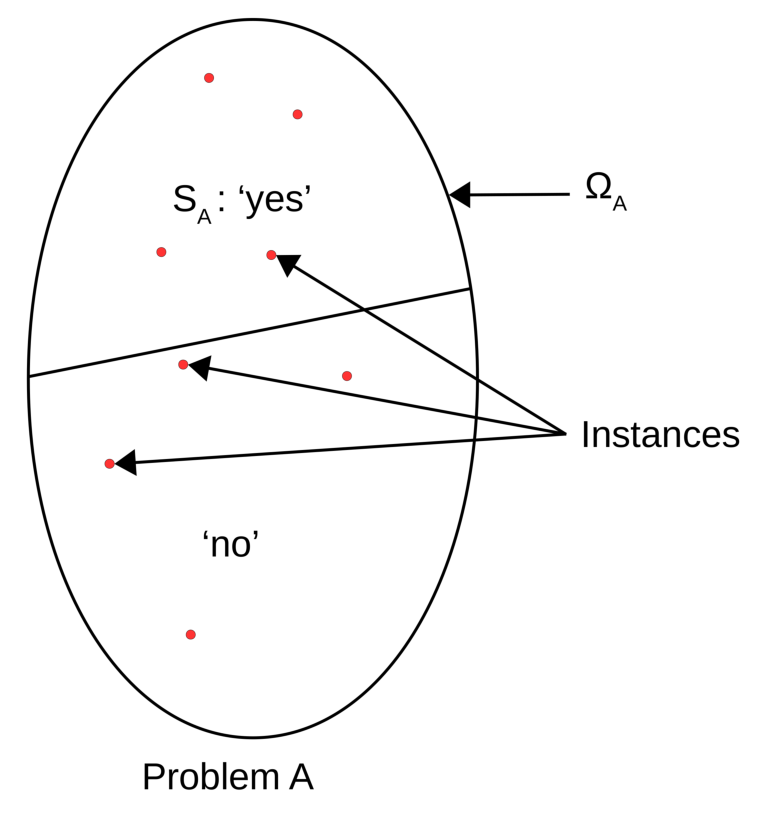
\includegraphics[width=.9\textwidth]{figures/problem.pdf}
    \caption{Algorithmic problem}
    \label{fig:problem}
  \end{subfigure}
  \begin{subfigure}[b]{0.5\textwidth}
    \centering
    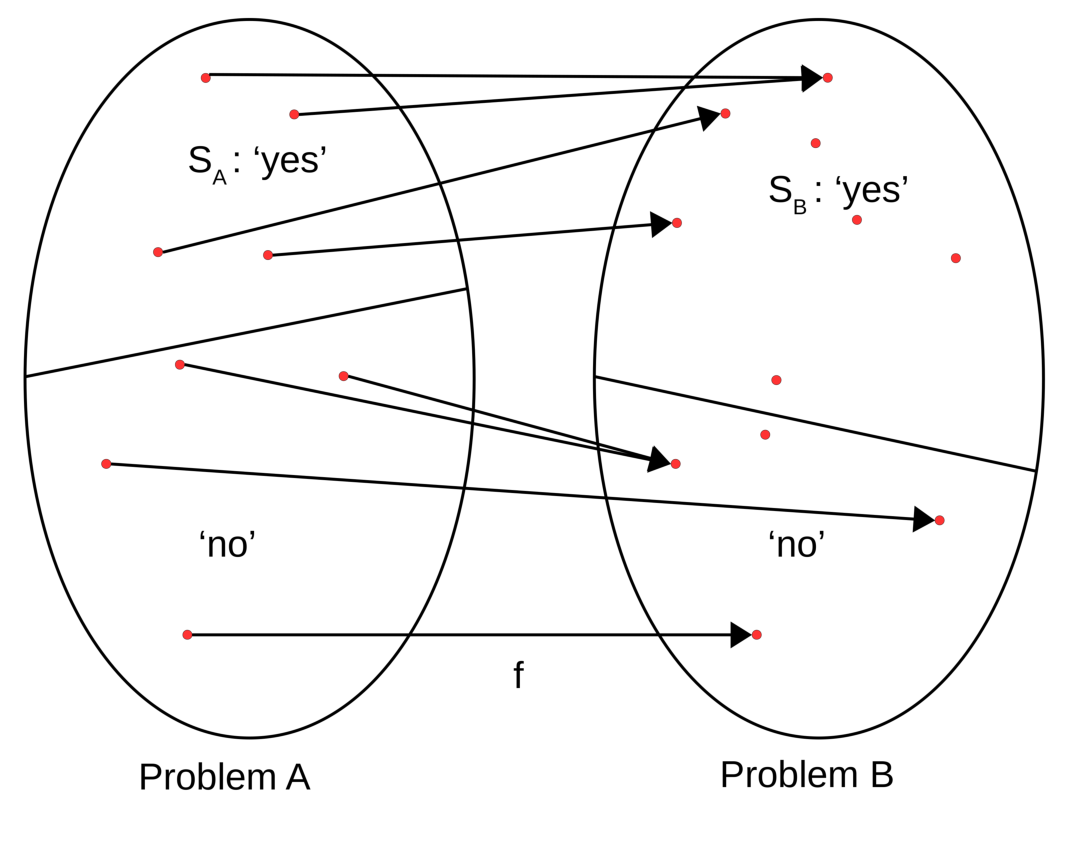
\includegraphics[width=\textwidth]{figures/reduction.pdf}
    \caption{Example of reduction}
    \label{fig:reduction}
  \end{subfigure}
%  \caption{Example of computation on the DAG}\label{fig:compute}
\end{figure}

The complexity class P is the class of problems for which there exists
a deterministic Turing machine deciding $S$ in a time polynomial to
the size of the instance. The complexity class NP consists of the
problems for which $S$ is accepted by a non-deterministic Turing
machine in polynomial time.

A reduction from a problem $A$ to a problem $B$ is a function
$f : \Omega_{A} \rightarrow \Omega_{B}$ such as for all instance
$\omega_{A}$ of $A$,
$\omega_{A} \in S_{A} \Leftrightarrow f(\omega_{a}) \in S_{B}$ (figure
\ref{fig:reduction}). As a result, if there exists a polynomial
reduction between $A$ and $B$ then $B$ is ``harder'' than $A$. Indeed,
if $S_{B}$ is accepted (respectively decided) by a Turing machine in
polynomial time, to accept (respectively decide) $S_{A}$ in polynomial
time, all there is to do is to apply the reduction to the instance of
$A$ and return the result computed by the Turing machine of the
problem $B$.
 
An algorithmic problem is called NP-hard if there exists a polynomial
reduction from each problem of the NP class to this one. The problems
that are both NP-hard and belong to the NP class are said to be
NP-complete.

\clearpage
\section*{Acknowledgments}

I would like to thank Christophe Godin for the time he spent
supervising and helping me, as well as him and Romain Azais for the
many discussions we had together about NP-completeness and Self-nestd
trees. I also would like to thank Frédéric Vivien, who helped me to
work on the first approach and gave me numerous advices on the way of
approaching a problem of NP-completness. 

\nocite{*}
\bibliographystyle{ieeetr}
\bibliography{biblio}


\end{document}
